%––––––––––––––––––––––––––––––––––––––––––––––––––––––––––––––––––––––––––––––––––––––%
%––––––––––––––––––––––––––––––––––––––––––––––––––––––––––––––––––––––––––––––––––––––%
%–––––––––––––––––––––––––––––    S E T T I N G S        ––––––––––––––––––––––––––––––%
%––––––––––––––––––––––––––––––––––––––––––––––––––––––––––––––––––––––––––––––––––––––%
%––––––––––––––––––––––––––––––––––––––––––––––––––––––––––––––––––––––––––––––––––––––%

\sloppy


% Options for packages loaded elsewhere
\PassOptionsToPackage{hyphens}{url}
%
\documentclass[12pt, a4paper, ngerman, bidi=default]{article}

%––––––––––––––––––––––––––––––––––––––––––––––––––––––––––––––––––––––––––––––––––––––%
%–––––––––––––––––––––––––––––    S E T T I N G S     ––––––––––––––––––––––––––––––%
%–––––––––––––––––––––––––––––      P A K E T E        ––––––––––––––––––––––––––––––%
%–––––––––––––––––––––––––––––
%––––––––––––––––––––––––––––––––––––––––––––––––––––––––––––––––––––––––––––––––––––––%
\usepackage[utf8]{inputenc}
\usepackage[T1]{fontenc}
\usepackage[fixed]{fontawesome5} %Fontawesome für Icons und Symbole; siehe https://mirrors.ibiblio.org/CTAN/fonts/fontawesome5/doc/fontawesome5.pdf
\usepackage{amsmath,amssymb}
\usepackage{tcolorbox}
\usepackage{afterpage}
\usepackage{graphicx}
\usepackage{subcaption} %Für die Verwendung von subfigure
\usepackage{setspace} %Für den Befehl \setstretch
\usepackage{transparent}
\usepackage{tikz}
  \usetikzlibrary{shapes.geometric, arrows.meta,fit, backgrounds, calc, positioning}
\usepackage{pgf-pie}%Für Kreisdiagramme
\usepackage{pgfplots}%Für Diagramme
  \pgfplotsset{compat=1.18}
\usepackage{eso-pic}%Für Hintergrundbilder
\usepackage{fvextra}    %Muss vor csquotes geladen werden
% \usepackage{csvsimple}%Für CSV-Dateien
% \usepackage{booktabs}   %für \toprule, \midrule, \bottomrule
% \usepackage{longtable}  %falls nicht schon geladen
% \usepackage{placeins}%Für \FloatBarrier
\usepackage[autostyle, german=quotes]{csquotes}
\usepackage[notes, backend=biber,language=ngerman, ibidtracker=context, citetracker=context, shorthandibid=true]{biblatex-chicago}
\DeclareDatamodelFields[type=field,datatype=literal]{software}
\DeclareDatamodelEntryfields[software]{title,author,date,version,url,urldate}
\DeclareBibliographyAlias{software}{misc}

\setlength{\skip\footins}{20pt}
\addbibresource{/Users/svenburkhardt/Developer/masterarbeit/1_MA_Arbeit/assets/Literature_Bib/Exportierte Einträge.bib}


% Optional:
\let\cite\footcite

\renewbibmacro*{date}{% 
    \ifentrytype{online}{% Falls der Eintrag @online ist, nimm das urldate
        \printtext[parens]{Zugriff am \usebibmacro{urldate}}}{\printdate}
    
}

\usepackage[ngerman]{babel}
\usepackage{pifont} %Für die Kästchen und Häkchen-Symbole
\usepackage[dvipsnames,svgnames,x11names,table]{xcolor}
%Zum Definieren und Verwenden von Farben
\definecolor{LightGray}{gray}{0.9}
\definecolor{UniRot}{HTML}{D20537}                  %Corperate Design Farben Uni Basel 
\definecolor{UniAnthrazit}{HTML}{46505A}            %Corperate Design Farben Uni Basel 
\definecolor{UniMint}{HTML}{A5D7D2}                 %Corperate Design Farben Uni Basel 
\definecolor{VeryLightGray}{gray}{0.95}%Sehr helles Grau
\definecolor{OldPaper}{HTML}{f4eade}


\definecolor{UniBlue}{HTML}{1F78B4}     %Kräftiges Blau
\definecolor{UniGold}{HTML}{FFB000}     %Goldgelb
\definecolor{UniViolet}{HTML}{6A3D9A}   %Violett

\definecolor{abbrev}{RGB}{255,153,153}             %Rot für Tags
\definecolor{add}{RGB}{204,255,238}                %Hellgrün/Türkis für Tags
\definecolor{sic}{RGB}{255,255,153}                %Hellgelb für Tags
\definecolor{unclear}{RGB}{255,230,184}            %Hellorange für Tags
\definecolor{date}{RGB}{153,153,255}               %Blau für Tags
\definecolor{organization}{RGB}{255,153,255}       %Pink für Tags
\definecolor{place}{RGB}{204,153,255}              %Lila für Tags
\definecolor{person}{RGB}{153,255,153}             %Hellgrün für Tags
\definecolor{signature}{RGB}{153,255,153}          %Hellgrün (gleiche Farbe wie Person) für Tags
\definecolor{eventTag}{HTML}{05A9FF}               %Blau für Tags
\definecolor{oldLetter}{RGB}{246,238,227}          %Beige für Hintergrund  
\definecolor{vscode-blue}{HTML}{569CD6}            %VSCode Blau für python
\definecolor{vscode-yellow}{HTML}{DCDCAA}          %VSCode Gelb für python
\usepackage{array}
\usepackage{minted}
\usepackage{wrapfig}
\usepackage{colortbl}
\usepackage{booktabs}
\usepackage[hyphens]{url}
\usepackage{ragged2e}
\usepackage[
  unicode=true,
  hyperfootnotes=true,
  colorlinks=true,
  linkcolor=Blue,
  filecolor=Maroon,
  citecolor=Blue,
  urlcolor=Blue,
  pdfborder={0 0 0}
]{hyperref}
\usepackage{nameref}
\usepackage{orcidlink}
\usepackage{iftex}
\ifPDFTeX
  \usepackage[utf8]{inputenc}
  \usepackage{lmodern}
  % Authblk, pdfpages etc. hier einbinden
\else
  \usepackage{fontspec}
\fi


% Use upquote if available, for straight quotes in verbatim environments
\IfFileExists{upquote.sty}{\usepackage{upquote}}{}

% Paragraph spacing configuration depending on the class
\makeatletter
\@ifundefined{KOMAClassName}{% if non-KOMA class
  \IfFileExists{parskip.sty}{%
    \usepackage{parskip}
 }{% else
    \setlength{\parindent}{0pt}
    \setlength{\parskip}{0pt}}
}{% if KOMA class
  \KOMAoptions{parskip=half}}
\makeatother


\usepackage[lmargin=2.5cm,rmargin=2.5cm,tmargin=2cm,bmargin=2cm]{geometry}
\setlength{\emergencystretch}{3em}%prevent overfull lines
\setcounter{secnumdepth}{-\maxdimen}%remove section numbering
% Make \paragraph and \subparagraph free-standing
\makeatletter
\ifx\paragraph\undefined\else
  \let\oldparagraph\paragraph%
  \renewcommand{\paragraph}{
    \@ifstar%
      \xxxParagraphStar%
      \xxxParagraphNoStar%
 }
  \newcommand{\xxxParagraphStar}[1]{\oldparagraph*{#1}\mbox{}}
  \newcommand{\xxxParagraphNoStar}[1]{\oldparagraph{#1}\mbox{}}
\fi
\ifx\subparagraph\undefined\else
  \let\oldsubparagraph\subparagraph%
  \renewcommand{\subparagraph}{
    \@ifstar%
      \xxxSubParagraphStar%
      \xxxSubParagraphNoStar%
 }
  \newcommand{\xxxSubParagraphStar}[1]{\oldsubparagraph*{#1}\mbox{}}
  \newcommand{\xxxSubParagraphNoStar}[1]{\oldsubparagraph{#1}\mbox{}}
\fi
\makeatother


\providecommand{\tightlist}{%
  \setlength{\itemsep}{0pt}\setlength{\parskip}{0pt}}\usepackage{longtable,booktabs,array}
\usepackage{calc}%for calculating minipage widths
% Correct order of tables after \paragraph or \subparagraph
\usepackage{etoolbox}
\makeatletter
\patchcmd\longtable{\par}{\if@noskipsec\mbox{}\fi\par}{}{}
\makeatother
% Allow footnotes in longtable head/foot
\IfFileExists{footnotehyper.sty}{\usepackage{footnotehyper}}{\usepackage{footnote}}
\makesavenoteenv{longtable}
\makeatletter
\def\maxwidth{\ifdim\Gin@nat@width>\linewidth\linewidth\else\Gin@nat@width\fi}
\def\maxheight{\ifdim\Gin@nat@height>\textheight\textheight\else\Gin@nat@height\fi}
\makeatother
% Scale images if necessary, so that they will not overflow the page
% margins by default, and it is still possible to overwrite the defaults
% using explicit options in \includegraphics[width, height, ...]{}
\setkeys{Gin}{width=\maxwidth,height=\maxheight,keepaspectratio}
% Set default figure placement to htbp
\makeatletter
\def\fps@figure{htbp}
\makeatother
% definitions for citeproc citations
\NewDocumentCommand\citeproctext{}{}
\NewDocumentCommand\citeproc{mm}{%
  \begingroup\def\citeproctext{#2}\cite{#1}\endgroup}
\makeatletter
%allow citations to break across lines
 \let\@cite@ofmt\@firstofone%
%avoid brackets around text for\cite:
 \def\@biblabel#1{}
 \def\@cite#1#2{{#1\if@tempswa, #2\fi}}
\makeatother
\newlength{\cslhangindent}
\setlength{\cslhangindent}{1.5em}
\newlength{\csllabelwidth}
\setlength{\csllabelwidth}{3em}
\newenvironment{CSLReferences}[2]%#1 hanging-indent, #2 entry-spacing
 {\begin{list}{}{%
  \setlength{\itemindent}{0pt}
  \setlength{\leftmargin}{0pt}
  \setlength{\parsep}{0pt}
 %turn on hanging indent if param 1 is 1
  \ifodd #1 \else%chktex 1
   \setlength{\leftmargin}{\cslhangindent}
   \setlength{\itemindent}{-1\cslhangindent}
  \fi
 %set entry spacing
  \setlength{\itemsep}{#2\baselineskip}}}
 {\end{list}}
\usepackage{calc}
\newcommand{\CSLBlock}[1]{\hfill\break\parbox[t]{\linewidth}{\strut\ignorespaces#1\strut}}
\newcommand{\CSLLeftMargin}[1]{\parbox[t]{\csllabelwidth}{\strut#1\strut}}
\newcommand{\CSLRightInline}[1]{\parbox[t]{\linewidth-\csllabelwidth}{\strut#1\strut}} %chktex 8
\newcommand{\CSLIndent}[1]{\hspace{\cslhangindent}#1}

\makeatletter
\@ifpackageloaded{caption}{}{\usepackage{caption}}
\AtBeginDocument{%
\ifdefined\contentsname%
  \renewcommand*\contentsname{Inhaltsverzeichnis}
\else
  \newcommand\contentsname{Inhaltsverzeichnis}
\fi
\ifdefined\listfigurename%
  \renewcommand*\listfigurename{Abbildungsverzeichnis}
\else
  \newcommand\listfigurename{Abbildungsverzeichnis}
\fi
\ifdefined\listtablename%
  \renewcommand*\listtablename{Tabellenverzeichnis}
\else
  \newcommand\listtablename{Tabellenverzeichnis}
\fi
\ifdefined\figurename%
  \renewcommand*\figurename{Abbildung}
\else
  \newcommand\figurename{Abbildung}
\fi
\ifdefined\tablename%
  \renewcommand*\tablename{Tabelle}
\else
  \newcommand\tablename{Tabelle}
\fi
}
\@ifpackageloaded{float}{}{\usepackage{float}}
\floatstyle{ruled}
\@ifundefined{c@chapter}{\newfloat{codelisting}{h}{lop}}{\newfloat{codelisting}{h}{lop}[chapter]}
\floatname{codelisting}{Listing}
\providecommand{\listoflistings}{\listof{codelisting}{Listingverzeichnis}}
\makeatother
\makeatletter
\makeatother
\makeatletter
\@ifpackageloaded{caption}{}{\usepackage{caption}}
\@ifpackageloaded{subcaption}{}{\usepackage{subcaption}}
\makeatother

% get rid of language-specific shorthands (see #6817):
\let\LanguageShortHands\languageshorthands%
\def\languageshorthands#1{}
\usepackage{bookmark}

\usepackage{placeins}                  %für \FloatBarrier
\usepackage[toc,page]{appendix}        %für eigene Anhangs-Umgebung
% optional:
% \usepackage{pdfcrypt}                  %für PDF-Passwortschutz

\IfFileExists{xurl.sty}{\usepackage{xurl}}{}%add URL line breaks if available
\urlstyle{same}%disable monospaced font for URLs
\hypersetup{
  pdftitle={Konzeption für AG Masterarbeit am
17.01.2025},
  pdfauthor={Sven Burkhardt},
  pdflang={de},
  colorlinks=true,
  linkcolor={blue},
  filecolor={Maroon},
  citecolor={Blue},
  urlcolor={Blue},
  pdfcreator={LaTeX via pandoc}
}

\usepackage{etoolbox}
\makeatletter
\providecommand{\subtitle}[1]{% add subtitle to \maketitle
  \apptocmd{\@title}{\par {\large #1 \par}}{}{}
}
\makeatother
\title{\vspace*{4cm} \LARGE Digitale Harmonie aus historischer Dissonanz
\color{UniMint} \rule{8cm}{1pt} \\  
\vspace{0.2cm}  
\color{white}\large Extraktion, Ordnung und Analyse\\unstrukturierter Archivdaten\\des Männerchor Murg}
\usepackage{etoolbox}
\makeatletter
\providecommand{\subtitle}[1]{% add subtitle to \maketitle
  \apptocmd{\@title}{\par {\large #1 \par}}{}{}
}
\makeatother
\subtitle{}
\author{Sven Burkhardt}
\date{2025-08-14}%chktex 8

%––––––––––––––––––––––––––––––––––––––––––––––––––––––––––––––––––––––––––––––––––––––%
%––––––––––––––––––––––––––––––––––––––––––––––––––––––––––––––––––––––––––––––––––––––%
%––––––––––––––––––––––––––––– T I T E L B L A T T   ––––––––––––––––––––––––––––––––––%
%––––––––––––––––––––––––––––––––––––––––––––––––––––––––––––––––––––––––––––––––––––––%
%––––––––––––––––––––––––––––––––––––––––––––––––––––––––––––––––––––––––––––––––––––––%
\begin{document}
\begin{titlepage}
    
% Setzt die Schriftfarbe auf Weiss
\color{white}
\pagecolor[HTML]{46505A} %Seitenfarbe in Uni Basel Anthrazit D20537 (rot)
\pagenumbering{gobble}   %Verhindert die Anzeige der Seitennummer auf dem Titelblatt
\date{}
\author{}
\maketitle
\begin{center}
  \author{\LARGE{\author{\vspace{-0.5cm}Sven Burkhardt}}}\\
  \vspace{4mm}
  \large{\orcidlink{0009-0001-4954-4426} {0009-0001-4954-4426}}\\%chktex 8%Orcid Link und Nummer
  \begin{figure}[h]
    \centering
    \color{white}
    \large{\href{https://dhlab.philhist.unibas.ch/en/persons/sven-burkhardt/}{{\hspace*{0.5mm}
\includegraphics[height=4.5
  mm]{./assets/Logos/Uni_basel_logo_white.png}}\hspace{3.4mm}\color{white} 17-056-912}}\\%chktex 8 %logo Unibas + Link + Immatrikulationsnummer
    \faIcon[regular]{calendar-alt}\date{\hspace*{2mm}15.08.2025}% chktex 8
  \end{figure}
  \setcounter{figure}{0}
\end{center}


% ------------ Hexagon grafik beginn -----------
\centering
\AddToShipoutPictureBG*{%
    \put(0,-40){%
        
\includegraphics[width=\paperwidth]{./assets/Logos/Hexagon_Deko}
  }
}
\centering
\AddToShipoutPictureBG*{%
    \put(0,810){%
        
\includegraphics[width=\paperwidth]{./assets/Logos/Hexagon_Deko}
   }
}
\centering
\AddToShipoutPictureBG*{%
    \put(33,752){%
        
\includegraphics[width=\paperwidth]{./assets/Logos/Hexagon_Deko}
   }
}
\centering
\AddToShipoutPictureBG*{%
    \put(-99,752){%
        
\includegraphics[width=\paperwidth]{./assets/Logos/Hexagon_Deko}
   }
}



\noindent%Verhindert Einzug des nachfolgenden Textes
% ------------ Hexagon grafik ende -----------



\begin{center}
    \vfill
    \begin{figure}
        \centering
        \begin{subfigure}{.3\textwidth}
          \centering
          
\includegraphics[width=.8\linewidth]{./assets/Logos/uni-basel-logo-en_white.png}
        \end{subfigure}%
        \begin{subfigure}{.3\textwidth}
          \centering
          
\includegraphics[width=.8\linewidth]{./assets/Logos/dhlab-logo-white.png}
        \end{subfigure}
        \end{figure}
        \setcounter{figure}{0}

    University of Basel\\
    Digital Humanities Lab\\
    Switzerland
\end{center}


\newpage
\color{black}          %Setzt die Schriftfarbe auf Schwarz für die folgenden Seiten
\setstretch{1.5}
\end{titlepage}
\newpage
%________________

%________________

%––––––––––––––––––––––––––––––––––––––––––––––––––––––––––––––––––––––––––––––––––––––%
%––––––––––––––––––––––––––––––––––––––––––––––––––––––––––––––––––––––––––––––––––––––%
%–––––––––––––––––––––––––––––   A B S T R A C T     ––––––––––––––––––––––––––––––––––%
%––––––––––––––––––––––––––––––––––––––––––––––––––––––––––––––––––––––––––––––––––––––%
%––––––––––––––––––––––––––––––––––––––––––––––––––––––––––––––––––––––––––––––––––––––%


\pagecolor{white}  
\color{black}  %Textfarbe zurücksetzen
\color{black} 
\setstretch{1.5}


\newpage 
Diese Arbeit befasst sich mit dem Archiv des Männerchor Murg in den Jahren des Zweiten Weltkrieges. 
Hierfür wird eine automatisierte Pipline auf Basis von LLMs und Patternmatching vorgestellt, mit deren Hilfe Named Entities extrahiert und weiterverarbeitet werden. 
Ziel ist es, dieses Archiv digital zugänglich, die beteiligten Personen sowie deren Netzwerke und dessen geographische Ausdehnung sichtbar zu machen.



%––––––––––––––––––––––––––––––––––––––––––––––––––––––––––––––––––––––––––––––––––––––%
%–––––––––––––––––––––––––––––      T A B L E        ––––––––––––––––––––––––––––––––––%
%–––––––––––––––––––––––––––––        O F            ––––––––––––––––––––––––––––––––––%
%–––––––––––––––––––––––––––––   C O N T E N T S     ––––––––––––––––––––––––––––––––––%
%––––––––––––––––––––––––––––––––––––––––––––––––––––––––––––––––––––––––––––––––––––––%



\newpage
\renewcommand*\contentsname{Inhaltsverzeichnis}%This controls the title of your table of contents.
{
\hypersetup{linkcolor=}
\setcounter{tocdepth}{5}%Sets the maximum sublevel to be displayed within the table of contents.
\tableofcontents
}
\pagenumbering{arabic}\setstretch{1.5}%Overwrites the previous command, pages are counted as normal from this point.


%––––––––––––––––––––––––––––––––––––––––––––––––––––––––––––––––––––––––––––––––––––––%
%––––––––––––––––––––––––––––––––––––––––––––––––––––––––––––––––––––––––––––––––––––––%
%––––––––––––––––––––––––      I N T R O D U C T I O N    ––––––––––––––––––––––%
%––––––––––––––––––––––––––––––––––––––––––––––––––––––––––––––––––––––––––––––––––––––%
%––––––––––––––––––––––––––––––––––––––––––––––––––––––––––––––––––––––––––––––––––––––%
\newpage
\section{Einleitung}
\subsection{Ziel und Relevanz der Arbeit}
\subsection{Formulierung der Forschungsfrage}
\subsection{Aufbau der Arbeit}
\subsection{Geografischer und historischer Kontext}
Die vorliegende Arbeit stützt sich auf Unterlagen aus dem Archiv des \enquote{Männerchor Murg} dessen Nachfolge im Jahr 2021 
durch die \enquote{New Gospelsingers Murg} angetreten wurde. Murg ist eine deutsche Gemeinde am Hochrhein, 
rund 30 km Luftlinie von Basel entfernt. Der Ort liegt am gleichnamigen Fluss Murg, der in den Rhein mündet. 
Beide Gewässer bildeten über Jahrhunderte hinweg den wirtschaftlichen Motor der Region: Die Wasserkraft der Murg 
begünstigte früh die Ansiedlung von Mühlen, Hammerwerken und Schmieden entlang des Bachlaufs, während der Rhein mit seiner 
Drahtseil-Fähre eine bedeutende Verkehrs- und Handelsverbindung bot, die bis zum Ersten Weltkrieg privat betrieben wurde.

Mit dem Ausbau der Landstrasse, der heutigen Bundesstrasse 34, sowie dem Anschluss an die Bahnstrecke Basel–Konstanz 
entwickelte sich Murg im 19. Jahrhundert von einer landwirtschaftlich geprägten Siedlung zu einer Gewerbe-, Handels- und 
Industriegemeinde. Die Wasserkraft wurde dabei zu einem entscheidenden Standortfaktor: Die Ansiedlung der Schweizer 
Textilfirma \textit{Hüssy \& Künzli AG} im Jahr 1853\cite[vgl.][]{gemeinde_murg_geschichte_nodate} trug wesentlich 
zum wirtschaftlichen Wachstum der Gemeinde bei. Zahlreiche Arbeitskräfte, vor allem aus der benachbarten Schweiz, 
machten Murg zu einem wichtigen Standort der regionalen Textilindustrie.

Die Gründung des \textit{Männerchor Murg} im Jahr 1861 durch Schweizer Textilarbeiter belegt diesen engen Zusammenhang 
zwischen wirtschaftlicher Migration, Industrialisierung und lokalem Vereinswesen. Diese historische Verflechtung bildet 
eine zentrale Grundlage für die vorliegende Untersuchung.


  

\newpage

%––––––––––––––––––––––––––––––––––––––––––––––––––––––––––––––––––––––––––––––––––––––%
%––––––––––––––––––––––––––––––––––––––––––––––––––––––––––––––––––––––––––––––––––––––%
%––––––––––––––––––––––––              Korpus            ––––––––––––––––––––––%
%––––––––––––––––––––––––––––––––––––––––––––––––––––––––––––––––––––––––––––––––––––––%
%––––––––––––––––––––––––––––––––––––––––––––––––––––––––––––––––––––––––––––––––––––––% 
\section{Korpus}
Aus dem Bestand des Ordners \textit{``Männerchor Akten 1925--1944''} werden für diese Arbeit ausschlieslich Akten verwendet, 
die während des Zweiten Weltkriegs verfasst wurden. Der Analysezeitraum erstreckt sich dementsprchend zwischen dem 01. September 1939 
und dem 8. Mai 1945, dem Tag der bedingungslosen Kapitulation Deutschlands.

Die zeitliche Eingrenzung ist notwendig, um die Funktionalität der im Folgenden beschriebenen Pipeline 
in einem klar definierten historischen Kontext demonstrieren zu können. Gleichzeitig führt diese Auswahl zu einer 
bewussten Reduzierung der potenziell erfassten Akteurinnen und Akteure, Orte und Organisationen. Diese Fokussierung ist 
insbesondere im Hinblick auf die Erstellung einer verlässlichen Groundtruth bedeutsam, die durch ergänzende Archivrecherchen 
mit historischen Metadaten angereichert wird.

Die Kombination aus einer präzise definierten Quellengrundlage und der digitalen Anreicherung dient dazu, das 
Potenzial der computergestützten Auswertung historischer Dokumente exemplarisch aufzuzeigen. 
Zugleich unterstreicht sie, dass die Qualität der Ergebnisse wesentlich von der sorgfältigen Eingrenzung 
des Korpus und der manuellen Validierung und Anreicherung abhängt.
%––––––––––––––––––––––––––––––––––––––––––––––––––––––––––––––––––––––––––––––––––––––%
%––––––––––––––––––––––––              Quellen            ––––––––––––––––––––––%
%––––––––––––––––––––––––––––––––––––––––––––––––––––––––––––––––––––––––––––––––––––––%

\subsection{Quellen}
\subsubsection{Quellentradierung}
In den Lagerräumen der New Gospel Singers Murg, dem Nachfolgeverein des Männerchors Murg, 
wird im Jahr 2018 mehrere je ca. 800 Seiten umfassende Ordner mit historischen Unterlagen gefunden. 
Für diese Arbeit wird ein Ordner mit der Aufschrift \textit{\enquote{Männerchor Akten 1925--1944}} gewählt, da er neben dem Ordner 
\textit{\enquote{Männerchor Akten 1946--1950}} den grössten Zeitraum abdeckt. Darüberhinaus bietet er das Potential, 
aufschlussreiche Einblicke in das Vereinsleben in der Zeit vor und während des Nationalsozialismus, insbesondere des Zweiten Weltkrieges, zu geben.\\ 
Der Ordner umfasst insgesamt 780 Seiten und deren Inhalt kann als \enquote{Protokoll}, \enquote{Brief}, \enquote{Postkarte}, \enquote{Rechnung}, 
\enquote{Regierungsdokument}, \enquote{Noten}, \enquote{Zeitungsartikel}, \enquote{Liste}, \enquote{Notizzettel} oder \enquote{Offerte} kategorisiert werden.


\subsubsection{Quellenbeschrieb}


\subsubsection{Datierung der Quelle}
blabla
Hier eine Grafik über die Verteilung im Ordner einfügen. 

\subsubsection{Dokumententyp}

\begin{figure}[htbp]
  \centering
  \begin{tikzpicture}
    \begin{axis}[
      ybar,
      bar width=20pt,
      ymin=0,
      ylabel={Anzahl Dokumente},
      symbolic x coords={Brief, Postkarte, Protokoll, Regierungsdokument, Zeitungsartikel, Rechnung, Offerte},
      xtick=data,
      nodes near coords,
      x tick label style={rotate=45, anchor=east},
      axis lines=left,
      enlarge x limits=0.15,
      grid=major,
      grid style={dashed, gray!30},
    ]
    \addplot[fill=gray!60] coordinates {
      (Brief,282) 
      (Postkarte,51) 
      (Protokoll,36) 
      (Regierungsdokument,5) 
      (Zeitungsartikel,4) 
      (Rechnung,1) 
      (Offerte,1)
    };
    \end{axis}
  \end{tikzpicture}
  \caption{Verteilung der Dokumententypen im untersuchten Bestand (150 Akten – 381 Seiten).}\label{fig:dokumententypen-bar}
\end{figure}



\subsubsection{Sichtung \& Kategorisierung in Akten}
blabla
% \paragraph{Inhalt???}
% blabla

\subsection{Digitalisierung der Quellen}

Die vorhandenen analogen Dokumente müssen zunächst fachgerecht für den Digitalisierungsprozess aufbereitet werden. 
Hierzu werden die Akten aus ihren ursprünglichen Ablagesystemen entnommen und sorgfältig von Heftklammern, Büro- und Gummibändern 
befreit. Diese konservatorischen Maßnahmen sind notwendig, um die langfristige Materialerhaltung zu gewährleisten, 
da insbesondere Korrosionsspuren ehemaliger Metallklammern die Papierfasern nachhaltig schädigen können. Zudem finden sich häufig 
Anzeichen von Säurefraß, sofern nicht säurefreies Archivmaterial verwendet wurde.

Für die eigentliche Digitalisierung kommt die native \enquote{Dateien}-Applikation von 
Apple\footnote{Vgl.\href{https://support.apple.com/de-de/guide/preview/prvw28034/mac}{Apple Support: Dateien-App}} zum Einsatz. 
Diese bietet neben einer vergleichsweise hochauflösenden Erfassung die Möglichkeit zur direkten Speicherung in einem Cloud-basierten 
Speichersystem sowie eine automatische Texterkennung (OCR). Ziel dieser Vorgehensweise ist es, die digitalisierten Inhalte möglichst 
schnell durchsuchbar zu machen und standortunabhängig für das Projekt zugänglich zu machen.

Die Aufnahme der Dokumente erfolgt mithilfe eines Tablets, das auf einem stabilen Stativ exakt im rechten Winkel (90\textdegree)
über dem zu digitalisierenden Schriftgut positioniert wird. Diese einfache, jedoch effiziente Konfiguration gewährleistet eine 
gleichbleibend hohe Bildqualität bei gleichzeitig hoher Verarbeitungsgeschwindigkeit. Die digital erfassten Dateien werden konsistent
 benannt und folgen einer vorab definierten Gesamtübersicht der Bestände. Mehrseitige Konvolute werden dabei als zusammengehörige 
 Akteneinheiten geführt, während Einzeldokumente entsprechend separat erfasst werden. Die Archivierung erfolgt sowohl analog als auch 
 digital auf Seitenebene, um eine möglichst feingranulare Erschließung zu ermöglichen.

Die initiale Speicherung erfolgt dabei standardmäßig im PDF-Format. Für die anschließende Verarbeitung mit den unten dargestellten 
Transkriptionswerkzeugen müssen die Dokumente jedoch in das JPEG-Format konvertiert werden. Die Umwandlung erfolgt automatisiert 
mithilfe eines eigens erstellten Python-Skripts, wie in Anhang~\ref{section:PDF_to_JPEG} beschrieben.\cite{burkhardt_githubpdf_to_jpegpy_2025}
Es extrahiert die Seiten, speichert im geeigneten 
Format ab und ergänzt die Dateinamen systematisch um eine dreistellige, führend nullengefüllte Seitennummer.

\subsection{Transkription}
Für die Transkrition der Daten wurde ein best-practise Ansatz gewählt. Nach Tests mit dem Python-Modul \textit{\enquote{Tesseract}} 
und unterschiedlichen LLMs wurde auf Transkribus zurückgegriffen. Eine Gegenüberstellung der drei erwähnten Tools findet 
sich im Kapitel~\nameref{section:Transkriptionen_Methoden}

\subsection{Tagging}
blabla
\subsubsection{Tagging mit Transkribus}
blabla
\subsubsection{Tagging mit LLM}
blabla
\subsection{Export}
blabla

%––––––––––––––––––––––––––––––––––––––––––––––––––––––––––––––––––––––––––––––––––––––%
%––––––––––––––––––––––––––––––––––––––––––––––––––––––––––––––––––––––––––––––––––––––%
%––––––––––––––––––––––––           Forschungsstand        ––––––––––––––––––––––%
%––––––––––––––––––––––––––––––––––––––––––––––––––––––––––––––––––––––––––––––––––––––%
%––––––––––––––––––––––––––––––––––––––––––––––––––––––––––––––––––––––––––––––––––––––% 

\subsection{Forschungsstand und Forschungslücke}\label{subsec:forschungsstand}
Die vorliegende Arbeit knüpft an mehrere Vorarbeiten an, die in den Jahren 2018 und 2022 am Departement Geschichte der Universität Basel durchgeführt
werden. In zwei Transkribus-Seminaren werden erste Teilbestände der \textit{Männerchor Akten 1925--1944} erschlossen und in einem Korpus
von 137 Einzeldokumenten zusammengeführt\cite[vgl.][]{burkhardt_feldpost_2022}.
Sie werden mit Metadaten versehen: Seitenlage im Ordner, Kurztitel und Entstehungsdatum, um die Grundlage für eine systematische Erschließung zu schaffen.

Während in einem frühen Projektschritt vorrangig häufig genannte Personennamen (\enquote{Carl Burger}, \enquote{Fritz Jung})
dokumentiert werden, richtet sich der Fokus im zweiten Schritt auf die Feldpost. Ziel ist es, über die Auswertung der Feldpostnummern
Rückschlüsse auf beteiligte Militäreinheiten, deren Stationierungen und Verlagerungen während des Zweiten Weltkriegs zu ziehen.

Für diese Recherchen kommen einschlägige Fachliteratur zu den jeweiligen Fachgebieten zum Einsatz. 
Hier sind besonders die Bücher von Alex Buchner\footcite[Vgl.][]{buchner_handbuch_1989}, Christian Hartmann\footcite[Vgl.][]{hartmann_wehrmacht_2010}, 
Werner Haupt\footcite[Vgl.][]{haupt_buch_1982}, Christoph Rass\footcite[Vgl.][]{rass_deutsche_2009}, Georg Tessin\footcite[Vgl.][]{tessin_verbande_1977} 
und Christian Zentner\footcite[Vgl.][]{zentner_illustrierte_1983} zu nennen.

Darüberhinaus werden eigene Recherchen in den Beständen des \textit{Bundesarchivs -- Militärarchiv Freiburg}\cite{hollmann_freiburg_2025} durchgeführt. Ergänzende Recherchen 
stammen aus den Suchlisten des \textit{Deutschen Roten Kreuzes (DRK)}\cite{reuter_drk_2025}. Hinzu kommen philatelistische Übersichts-Websites \cite{noauthor_feldpost_nodate}, 
die bei der Entzifferung von Briefmarken und Stempeln helfen.
Absoult essentiell für den Erfolg dieser Recherchen sind Citizen-Science-Foren\footnote{vor Allem werden verwendet: 
\textit{Forum der Wehrmacht}~\parencite{hermans_forum_nodate} und das \textit{Lexikon der Wehrmacht}~\parencite{altenburger_lexikon_nodate}.}. Sie ergänzen und validieren eigene Forschung.

Parallel zur inhaltlichen Erschließungen entsteht 2022 eine erste digitale Storymap mit \textit{ArcGIS},
die zentrale Ergebnisse des Projekts öffentlich zugänglich macht. Grundlage bildet die Sichtung, konservatorische Aufbereitung und Digitalisierung
von zunächst rund 30 der etwa 800 Seiten Vereinsakten. Der Teilkorpus wird entheftet, gescannt und mit Metadaten wie Absender, Datum,
Feldpostnummer und Einheit versehen. Da jedes Dokument einen anderen Verfasser aufweist, erfolgt die Transkription manuell. Eine automatische Handschriftenerkennung 
ist aufgrund der heterogenen Schriftbilder nicht praktikabel.
Am Beispiel einzelner Sänger wie \textit{Emil Durst} lässt sich durch die Rechercheergebnisse mithilfe der Feldpostnummern und ergänzender Kartenmaterialien der Aufenthaltsort
bis auf Gebäude oder wenige Meter genau rekonstruieren. Diese Erkenntnisse werden mit historischen Karten, Luftbildern und Ortsrecherchen verknüpft
und in einer interaktiven ArcGIS-Karte visualisiert, die Stationierungen, Märsche und Frontverschiebungen der Chormitglieder anschaulich darstellt. 

Die in diesen Vorprojekten erarbeiteten Listen, Geodaten, Transkriptionen und Visualisierungen fließen in die vorliegende Arbeit ein
und bilden eine wesentliche Grundlage für die erweiterte, automatisierte Pipeline, die im Folgenden vorgestellt wird. Dazu gehören beispielsweise auch die Verbandsabzeichen, 
Taktische Zeichen\cite[vgl][S.64-66]{haupt_buch_1982} der jeweiligen Einheiten, die auch in die Groundtruth der vorliegenden Arbeit inkorporiert werden.

Abgesehen von diesen Vorarbeiten ist der Quellenkorpus wissenschaftlich unerschlossen. Mit dieser Arbeit liegt erstmals eine
umfassendere wissenschaftliche Auswertung vor.

Mit der notwendigen manuellen Recherche in oben dargelegten Datenbankstrukturen wird zugleich sichtbar, wie sehr es an Brücken fehlt, 
um unterschiedliche Klassifikationen, fachspezifische Ordnungslogiken und semantische Webtechnologien nachhaltig miteinander zu verbinden. Ein verhältnismässig einfaches
Webscraping nach Informationen zu diesem Korpus ist nahezu unmöglich. Ausgeführt werden diese Probleme beispielsweise bei 
Smiraglia und Scharnhorst (2021)\cite[vgl.][]{richard_linking_2022}, 
 die anhand konkreter Fallstudien verdeutlichen, wie fragmentiert semantische Strukturen bislang entwickelt werden 
 und welche Hürden bei der praktischen Verknüpfung heterogener Wissensorganisationen bestehen. Dabei benennen sie insbesondere die 
 Herausforderungen bei der Übersetzung historisch gewachsener Klassifikationen in standardisierte semantische Formate, 
 die Notwendigkeit dauerhafter technischer Wartung und die Abhängigkeit von nachhaltigen Infrastruktur-Partnern\cite[vgl.][Kap.~2 und 5]{richard_linking_2022}.

Für eine Einordnung zu historischen Netzwerkanaylsen sei auf Gamper\&Reschke \cite{gamper_knoten_2015} verwiesen. Der Sammelband
\textit{Knoten und Kanten III} verdeutlicht, dass die historische Netzwerkanalyse zwar von einem interdisziplinär etablierten Methodenkanon 
profitiert, jedoch nach wie vor vor erheblichen Herausforderungen steht. Dazu zählen die Fragmentierung historischer Quellen, der hohe manuelle 
Erfassungsaufwand und methodische Desiderate im Umgang mit zeitlichen und räumlichen Dimensionen. Erschwerende Faktoren einer systematische Erfassung 
relationaler Strukturen. Dennoch eröffnen netzwerkanalytische Verfahren – besonders im Zusammenspiel mit relationaler Soziologie 
und Figurationsansätzen – neue Perspektiven auf Macht, Abhängigkeiten und Akteurskonstellationen in historischen Gesellschaften.





%––––––––––––––––––––––––––––––––––––––––––––––––––––––––––––––––––––––––––––––––––––––%
%––––––––––––––––––––––––––––––––––––––––––––––––––––––––––––––––––––––––––––––––––––––%
%––––––––––––––––––––––––           Methodisches Vorgehen        ––––––––––––––––––––––%
%––––––––––––––––––––––––––––––––––––––––––––––––––––––––––––––––––––––––––––––––––––––%
%––––––––––––––––––––––––––––––––––––––––––––––––––––––––––––––––––––––––––––––––––––––% 
\section{Methodisches Vorgehen}
\subsection{Genutze Tools}
Digitale Methoden spielen für die Durchführung dieser Arbeit eine zentrale Rolle. Von der Digitalisierung der Quellen
über die Transkription bis hin zur Auswertung durchlaufen die Daten zahlreiche Prozessschritte, die mithilfe von Large 
Language Models, Deep-Learning-Modellen und anderen digitalen Werkzeugen verarbeitet und visualisiert werden. 
Die Auswahl der Tools orientierte sich dabei an Kriterien wie Verfügbarkeit (Open~Source vs.\ proprietär), 
Kompatibilität, Community-Support, erforderlichem Arbeitsaufwand und selbstverständlich dem konkreten Mehrwert für 
die Forschungsfragen.

In diesem Kapitel werden sowohl Werkzeuge vorgestellt, die tatsächlich eingesetzt wurden, als auch solche, die sich 
im Verlauf des Projekts als ungeeignet erwiesen. Transparenz ist hierbei ein wesentlicher Aspekt: Ein grosser Teil der 
Methodik entwickelte sich erst im Forschungsprozess selbst. Da sich Large Language Models rasant weiterentwickeln, 
ist nicht immer von Beginn an klar, ob ein Tool für den eigenen Anwendungsfall geeignet ist.
Um diese Unsicherheiten zu dokumentieren, werden hier auch gescheiterte Versuche dargestellt.

\subsubsection{LOD – Linked Open Data}

Linked Open Data (LOD) bezeichnet einen dezentral organisierten Ansatz zur Veröffentlichung und 
Verknüpfung strukturierter Daten im Web. Ziel ist es, Datensätze verschiedener Institutionen und Akteure 
maschinenlesbar zugänglich zu machen und über standardisierte Formate wie RDF und SPARQL miteinander zu 
verbinden\cite[ vgl.][Preface S. VI \& S. 13f]{garoufallou_metadata_2020}. 
Wesentliches Merkmal der LOD-Cloud ist dabei die Nutzung semantischer Beziehungen, insbesondere Äquivalenzen einzelner Daten. 
Hierfür wird häufig das Prädikat \texttt{owl:sameAs} genutzt, um z.B. mit \colorbox{VeryLightGray}{\textit{:Choir owl:sameAs wd:Q131186}} eine eigene 
Instanz als identisch mit der Wikidata-Entität für einen Chor zu deklarieren.
Klassen oder Instanzen können so aus unterschiedlichen Datenquellen eindeutig identifiziert und zusammengeführt werden.

Die OWL Web Ontology Language, entwickelt vom World Wide Web Consortium (W3C), ist damit ein zentrales Werkzeug für die Realisierung von 
LOD.\cite[ vgl.][]{smith_owl_2004} 
Mit ihr lassen sich Ontologien definieren, die Domänen über Klassen, Individuen und deren Relationen formal beschreiben. 
Sie ermöglichen, logische Schlussfolgerungen zu ziehen, um verteilte Datenbestände zu verknüpfen und maschinenlesbar auszuwerten.
Besonders relevant ist dabei \texttt{owl:sameAs}, das als Identitätsrelation fungiert: 
Es deklariert Instanzen, die in unterschiedlichen Quellen unter verschiedenen URIs\footnote{Abk. URI\: Uniform Resource Identifier} geführt werden, 
als dasselbe reale Objekt\cite[ vgl.][2.3. Data Aggregation and Privacy]{smith_owl_2004}
und ermöglicht so eine präzise Zusammenführung von Informationen — ein Grundpfeiler für die Interoperabilität im Semantic Web.
Die OWL-Spezifikation baut auf RDF\footnote{Abk. RDF\; Resource Description Framework} auf und erweitert es um zusätzliche Konzepte.
Die RDF-Daten werden häufig im Turtle-Format (TTL) serialisiert, einer textbasierten Notation für RDF, die eine kompakte, leicht lesbare Schreibweise bietet.
Dieses Format eignet sich besonders für den Austausch und die manuelle Bearbeitung von RDF-Tripeln.
Die Sprache liegt in drei Varianten vor\footnote{OWL Lite, OWL DL und OWL Full}, die sich im Grad ihrer Ausdrucksstärke 
unterscheiden.\cite[ vgl.][1.1. The Species of OWL.]{smith_owl_2004}
Insbesondere OWL DL bietet einen praktikablen Mittelweg zwischen hoher Ausdruckskraft und vollständigem, entscheidbarem Schliessen (Reasoning) 
und ist daher für viele LOD-Anwendungsfälle geeignet.

Trotz ihres Potenzials wird diese Form der Datenverknüpfung bislang jedoch nicht von allen Websites konsequent 
umgesetzt.\cite[ vgl.][S. 14]{garoufallou_metadata_2020}. Für die technische 
Umsetzung für diese Arbeit werden zwei zentrale Werkzeuge genutzt: Protégé zur Modellierung der Ontologie und GraphDB für deren Verwaltung und Abfrage.

\paragraph{Protégé} Zur praktischen Modellierung der Ontologie kam \textit{Protégé} zum Einsatz. 
Protégé ist eine weit verbreitete Open-Source-Software zur Erstellung, Visualisierung und Verwaltung von Ontologien.
Die grafische Oberfläche unterstützt eine intuitive Klassendefinition, 
Relationserstellung und Instanzverwaltung. 
Mit Hilfe von Plugins können darüber hinaus logische Konsistenzprüfungen durchgeführt und 
Ontologien direkt im OWL-Format exportiert werden, um sie in LOD-Workflows einzubinden.
Die initiale Version der Ontologie für dieses Projekt entstand zuerst im Codeeditor \textit{Visual Studio Code} wurde aber schnell vollständig in Protégé überarbeitet.
Damit bildet das Programm die Grundlage für erste Experimente mit Abfragen in SPARQL.

\paragraph{GraphDB} Für die Speicherung und Abfrage der Ontologie wurde \textit{GraphDB} verwendet. 
GraphDB ist eine spezialisierte RDF-Triplestore-Datenbank, die es ermöglicht, 
grosse Mengen an semantisch verknüpften Daten effizient zu verwalten. 
Mit der integrierten SPARQL-Schnittstelle können Benutzer gezielt nach Instanzen, Klassen und Relationen suchen 
und komplexe Muster in den Datenbeständen erkennen. 
Im Rahmen dieser Arbeit diente GraphDB als Backend, um die in Protégé entwickelte Ontologie zu testen 
und mit realen Entitäten aus den untersuchten Quellen abzugleichen.


\paragraph{mmma-Ontologie}\\

\begin{minipage}{0.48\textwidth}% Linke Box = TEXT
Ein wichtiger Aspekt dieser Arbeit ist die Unstrukturiertheit relevanter Informationen. 
Aus diesem Grund wurde auf der Basis der Oben beschrieben Semantik begonnen, eine eigene Ontologie zu entwickeln, die die identifizierten Entitäten systematisch erfasst\footnotemark
Beim Schreiben dieser initialen Ontologie aus rund 2000 Zeilen Code erweist sich schnell ein neues Problem. Die Datengrundlage aus den geschilderten Vorprojekten (siehe~\nameref{subsec:forschungsstand}) ist 
zu klein, um daraus eine aussagekräftige Netzwerkanalyse zu machen. Hierfür erweisen sich die Unterschiede der Daten zusätzlich als zu gross tische Grundlage des Globalund damit aufwendig. Der Fokus der Arbeit verschiebt sich dementsprechend von der Ontologieentwicklung 
auf die Extraktion von Entitäten.
\end{minipage}%
\hfill%
\begin{minipage}{0.48\textwidth}% Rechte Box = BILD
  \centering
  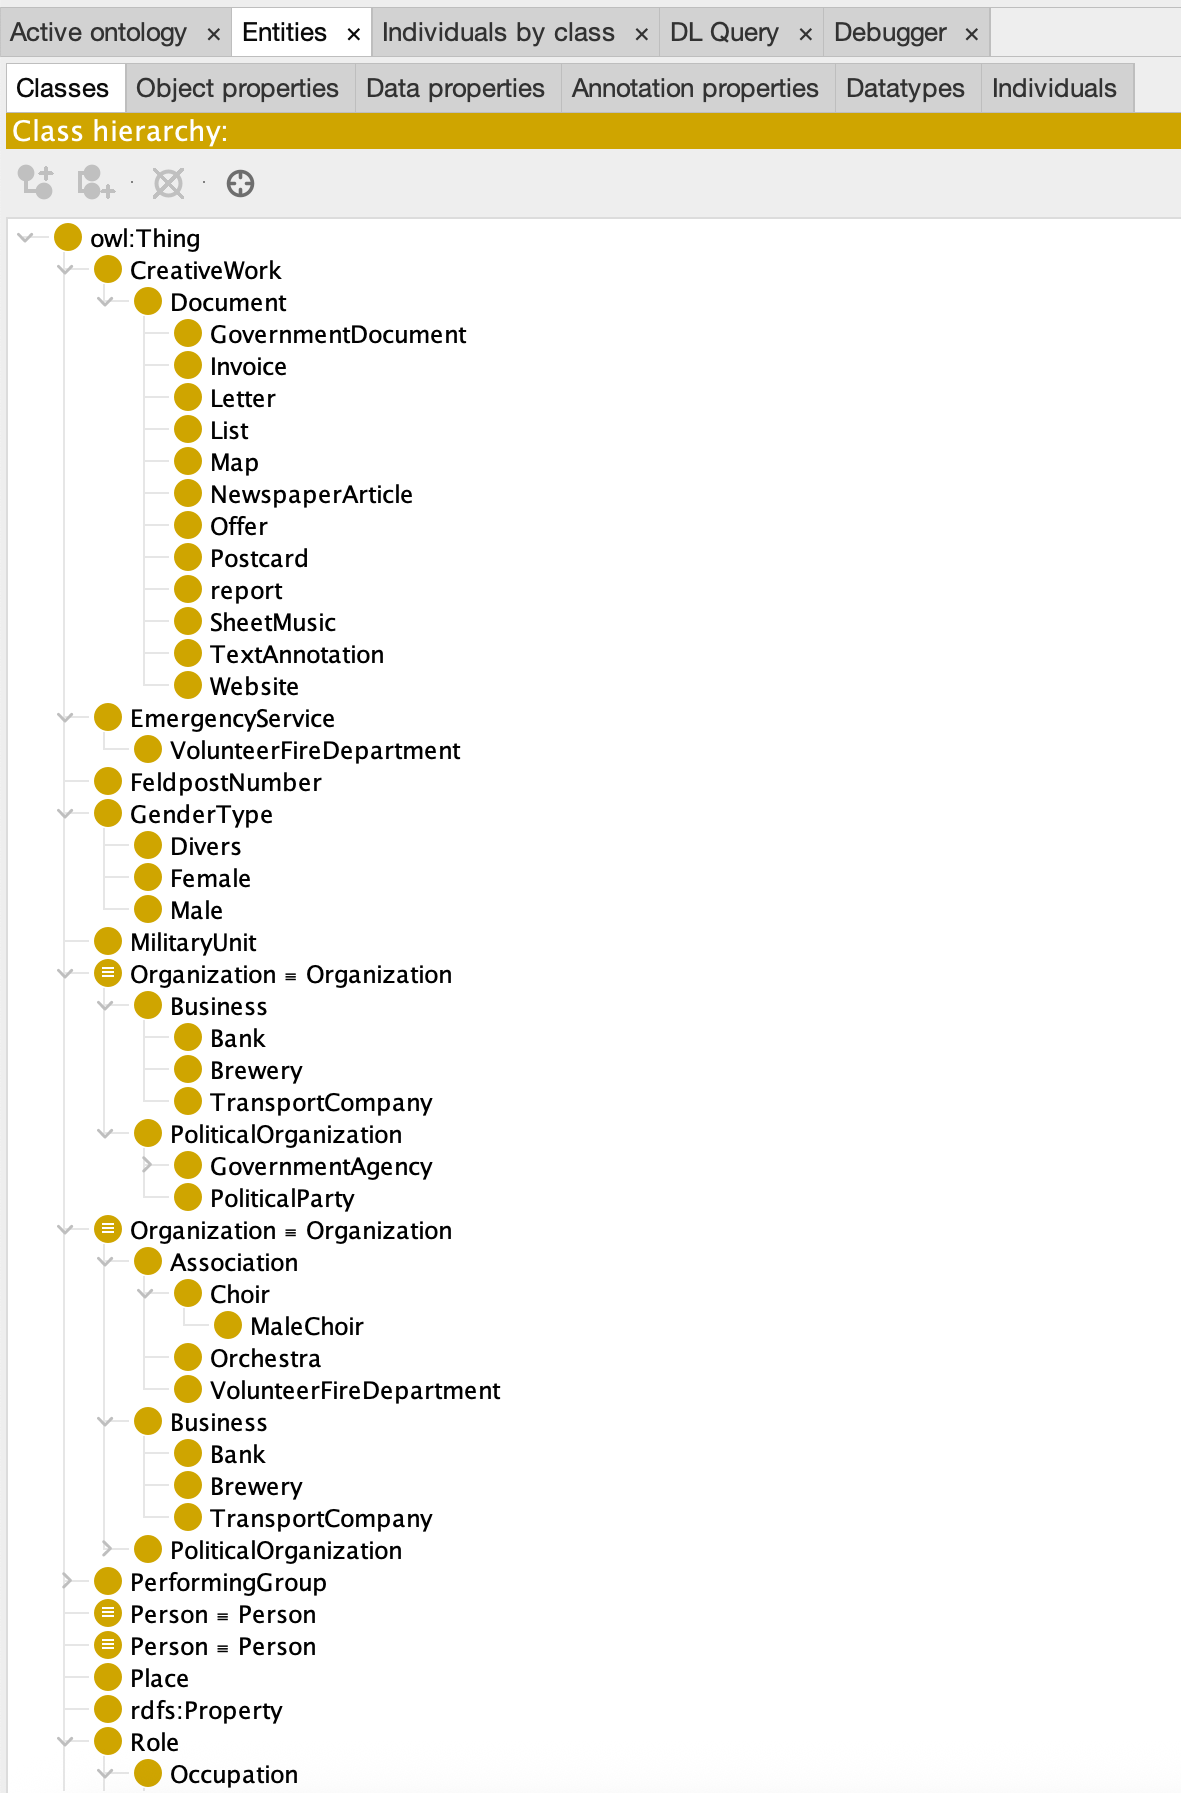
\includegraphics[width=\linewidth]{assets/Images/Bildschirmfoto_ttl_ontologie_Ausschnitt.png}
  \captionof{figure}{Ausschnitt der TTL-Ontologie.}\label{fig:ttl-ontologie}
\end{minipage}
\footnotetext{Abk.\ mmma; Männerchor Murg MasterArbeit.}


\vspace{1em}

Der bestehende Datensatz ist zu klein, um eine umfangreiche Ontologie lohnend zu machen. Hinzu kommen externe Quellen, und deren Zugänglichkeit. Zuverlässige Quellen für Informationen 
über militärische Einheiten und deren Feldpostnummern sind das \enquote{Forum der Wehrmacht}\cite[ vgl.][]{altenburger_lexikon_nodate} 
und der \enquote{Suchdienst des DRK}\cite[ vgl.][]{reuter_drk_2025}. In beiden Fällen liegen die Daten jedoch nicht als LOD vor, sondern im Forum als einfache Strings 
und beim Deutschen Roten Kreuz als OCR-PDF\footnote{OCR = Optical Character Recognition} historischer Suchlisten aus der Nachkriegszeit. Ein manuelles Recherchieren dieser Daten scheint zu diesem Zeitpunkt
den Rahmen der Arbeit zu sprengen. Die in diesem Schritt geleistete Vorarbeit beim Sortieren und Klassifizieren von Entitäten, besonders in Verknüpfung mit selbst erstellten Wikidata-Klassen 
wird in späteren Prozessschritten wieder aufgegriffen\footnote{siehe Kapitel Nodegoat}.

\subsubsection{Wikidata}

\textit{Wikidata}\cite[vgl.][]{noauthor_wikidata_nodate} ist eines der zentralen Repositorien für Linked Open Data, und bietet eine hohe Interoperabilität durch standardisierte
URIs, SPARQL-Endpunkte und offene APIs zu den Entitäten.
Jede Entität erhält dabei eine eindeutige, persistente URI 
(z.B. \colorbox{VeryLightGray}{\textit{wd:Q131186}} für einen Chor), die in LOD-Szenarien 
als stabiler Referenzpunkt dient.
Neben anderen betonen Martinez \& Pereyra Metnik (2024) beispielsweise: \\
\textit{\enquote{Wikidata stands out for its great potential in interoperability and its ability to connect data from various domains.}}\cite{martinez_comparative_nodate}

Wikidata entspricht, ebenso wie das nachfolgend beschriebene GeoNames, den FAIR-Prinzipien: Die Daten sind 
\textbf{F}\textit{indable} und \textbf{A}\textit{ccessible}, \textbf{I}\textit{nteroperable} und \textbf{R}\textit{eusable}\cite[ vgl.][S. 2]{wilkinson_fair_2016}.

Im Rahmen dieser Arbeit dient Wikidata als zentrale externe Referenz, um lokal erhobene Entitäten mit international etablierten Datenobjekten 
zu verknüpfen und so ihre Interoperabilität sicherzustellen. Die Plattform ermöglicht eine eindeutige Identifizierung sowie die maschinenlesbare 
Anreicherung um zusätzliche Informationen.

Die praktische Umsetzung zeigt jedoch eine strukturelle Einschränkung. Für diese Arbeiteigens angelegter Einträge auf Wikidata werden
trotz systematischer Verknüpfung mit anderen dort verwalteten Entitäten, etwa mit Armeen, Militäreinheiten, Orten und Personen, entfernt die Community–Moderation etwa 70\% dieser Einträge. 
Das zeigt einerseits hohe internen Qualitätsanforderungen auf, andererseits werden diese jedoch nicht klar kommuniziert. Mit regidem Löschen neuer Einträge wird die Verlässlichkeit und den Nutzen der 
geleisteten Arbeit erheblich begrenzt. 
Aufwand und Unsicherheit über die Persistenz der Einträge machen den ursprünglich vorgesehenen LOD–Ansatz in dieser Form nicht praktikabel.

\subsubsection{GeoNames}

Ebenso wie Wikidata bietet \textit{GeoNames}\cite[vgl.][]{noauthor_geonames_nodate} eine Open-Source-Plattform für interoperable Daten. GeoNames fokussiert sich hierbei auf geografische Informationen 
und stellt eine umfassende Datenbank mit über 25 Millionen Ortsnamen und rund 12 Millionen eindeutigen geografischen Objekten bereit.  
Alle Einträge sind in neun Feature–Klassen und über 600 spezifische Feature–Codes kategorisiert. Die Plattform integriert Daten zu 
Ortsnamen in verschiedenen Sprachen, Höhenlagen, Bevölkerungszahlen und weiteren Attributen aus unterschiedlichen nationalen und internationalen Quellen.  
Sämtliche Geokoordinaten basieren auf dem WGS84–System\footcite[\textit{WGS84: geodätische Grundlage des Global Positioning System (GPS)}; vgl.][]{noauthor_wgs84_nodate}
und können über frei zugängliche Webservices oder eine API abgerufen werden.  
Darüber hinaus erlaubt GeoNames registrierten Nutzenden, bestehende Datensätze über eine Wiki–Oberfläche zu bearbeiten oder zu ergänzen, wodurch eine 
kollaborative Qualitätssicherung gewährleistet wird.

GeoNames wird in dieser Arbeit intensiv zur Referenzierung von Ortsnamen verwendet und bildet die Basis für die Groundtruth, wie sie in den Kapiteln \textit{Nodegoat} und 
\textit{place\_matcher.py} beschrieben ist. Im Gegensatz zu Wikidata wurde hier von Beginn an darauf verzichtet, eigene Ortsdatensätze zu ergänzen. Dies liegt einerseits an 
den klar kommunizierten Community–Guidelines und andererseits daran, dass der Datensatz bis auf wenige, sehr lokale Flurnamen als nahezu vollständig gilt.

Historische Gebäude wie Gaststätten oder Spitäler fehlen folgerichtig in der GeoNames–Datenbank. Diese Lücke ist erwartbar, aber erwähnenswert, da GeoNames 
ansonsten eine nahezu vollständige und ausgesprochen detaillierte Datengrundlage bietet.

\subsubsection{Transkriptionen (Methodenvergleich)}\label{section:Transkriptionen_Methoden}
\paragraph{Tesseract}

war scheisse

\paragraph{LLM}

war scheisse und manipulativ

\paragraph{Transkribus}

Transkribus ist eine webbasierte Plattform zur automatisierten Handschrifterkennung (HTR) und Texterkennung (OCR), die sich seit ihrer Entwicklung im EU-Projekt READ (Recognition and Enrichment of Archival Documents)\cite[vgl.][]{noauthor_recognition_nodate} als Standardwerkzeug in den digitalen Geschichtswissenschaften etabliert hat \cite[vgl.][postnote]{muhlberger_transkribus_2019}. Betrieben wird Transkribus durch die READ-COOP SCE, einer europäischen Genossenschaft.

Für die vorliegende Arbeit wird sowohl die Webanwendung \textit{\enquote{Transkribus Lite}} als auch der \textit{Desktop-\enquote{Transkribus Expert Client}} genutzt. Letzterer ist eine Fortführung der ursprünglichen, im Rahmen des READ-Projekts entwickelten Software. Die Verwendung des Expert Clients in Kombination mit \textit{FileZilla Pro} als FTP-Client ermöglicht es, die grosse Zahl an Scanseiten effizienter in das Transkribus-Dateimanagement einzupflegen. Die für das Projekt nötige Scholar-Lizenz wird über RISE der Universität Basel\cite[weitere Informationen:][postnote]{decker_home_nodate} bezogen.

Neben der eigentlichen Transkription bietet Transkribus die Möglichkeit, Named Entities wie Personen, Orte, Organisationen und Datumsangaben direkt im Dokument zu annotieren. Dies geschieht über eine umfangreiche Tagging-Funktion, die neben struktureller Tags wie Abkürzungen (\enquote{abbrev}) auch individuell erweiterbar sind. Für diese Arbeit wird beispielsweise der Custom-Tag \colorbox{signature}{\texttt{signature}} eingeführt, der dem Anhang entnommen werden können.

Nach erfolgter Bearbeitung stellt Transkribus Funktionen zur Verfügung, die Transkriptionen inklusive Tags als strukturiertes Markup im XML-Format zu exportieren.

In der praktischen Anwendung zeigt sich jedoch eine erhebliche Diskrepanz zwischen den vorgesehenen Funktionen und der tatsächlich umgesetzten Exportlogik. Die händisch markierten und ausformulierten Abkürzungen werden im generierten Page-XML nicht ausgegeben, sodass diese Information für eine weitergehende Auswertung verloren geht. 

Aus Abkürzungen wie V.D.A soll in XML \colorbox{VeryLightGray}{\textless abbrev expansion=\enquote{Verein für das Deutschtum im Ausland}\textgreater V.D.A.\textless /abbrev\textgreater} werden. Tatsächlich fehlt der Tag komplett, V.D.A wird zum einfachen String. Unter Umständen wird dieser nun von den LLMs nicht mehr als Organisation erkannt. 

Besonders gravierend ist das Defizit bei der Handhabung von Listen. Zwar können Listenobjekte innerhalb der Benutzeroberfläche manuell angelegt und befüllt werden, beim Export bleibt die zugehörige XML-Struktur jedoch leer. Ein technischer oder benutzerfreundlicher Workaround, um diese Daten maschinenlesbar zu extrahieren, existiert bislang nicht. Um auf die Listeninhalte im XML nicht zu verzichten, müssen sie daher als regulärer Fliesstext markiert werden — mit dem Effekt, dass die logische Gliederung, die etwa für Mitgliederverzeichnisse, Inventarlisten oder Aufstellungen forschungsrelevant ist, systematisch verloren geht. Dies führt zu erheblichem Mehraufwand und stellt eine signifikante methodische Limitation dar, insbesondere für Vorhaben, die auf einer automatisierten Weiterverarbeitung konsistenter Strukturdaten beruhen. Hinzu kommt der grosse Zeitaufwand für die manuelle Listengestaltung, die letztlich nicht zielführend verwertet werden kann.

Die Herausforderungen decken sich mit den Beobachtungen von Capurro et al.\cite[][]{capurro_experimenting_2023}, die in ihrem Experiment mit einem mehrsprachigen und multi-autoren Handschriftenkorpus ebenfalls auf erhebliche Grenzen von Transkribus hinweisen: Sowohl die automatische Layout-Erkennung als auch die Handhabung komplexer Dokumentstrukturen erwiesen sich als fehleranfällig und machten umfangreiche manuelle Nachbearbeitung unvermeidbar. Auch der Versuch, HTR-Ergebnisse\footnote{Abk.: \textbf{HTR}, Handwritten Text Recognition} nachträglich automatisch zu verbessern (Postcorrection), brachte keine Verbesserung der Fehlerquote. Damit bestätigt sich der Befund, dass ein projektspezifisch trainiertes Modell – wie es hier mit vier Trainings-Iterationen umgesetzt wurde – zwar die CER senken kann, strukturelle Probleme jedoch ungelöst bleiben.

Der methodische Mehrwert von Transkribus liegt trotz dieser Limitierungen in der Möglichkeit, ein eigenes, auf den spezifischen Handschriftencorpus angepasstes HTR-Modell zu trainieren. Ein generisches Modell \textit{(The German Giant I)} erzielt zu Beginn eine Character Error Rate \textit{(CER)} von 8,3\%. Durch das Training auf einer eigens erstellten Groundtruth mit 149 Seiten lässt sich ein projektspezifisches Modell entwickeln, das die CER auf 6,58\% senkt. Auch für das Tagging selbst wurde eine umfassende Groundtruth für etwaige spätere Anwendungen (und als Vergleich für die LLMs) erstellt. Sie besteht aus insgesamt 100 Seiten händischer Annotation. Diese umfassende manuelle Nachbearbeitung stellt ein möglichst konsistentes, maschinenlesbares XML sicher. Aus diesem Grund werden auch Taggingregeln festgehalten, die später auch an das LLM weitergegeben werden.

Insgesamt zeigt sich, dass Transkribus als Plattform eine sehr hilfreiche Basis für grossvolumige Transkriptionsprojekte bietet. Die automatisierte Erkennung spart erhebliche Zeit, ersetzt jedoch weder editorische Sorgfalt noch eine manuelle Qualitätssicherung. Gerade für Forschungsprojekte, die auf präzisen Strukturdaten beruhen, wie hier für Netzwerkanalysen mit Nodegoat, bleibt eine kritische Reflexion der Tool-Limitierungen unerlässlich. Transkribus unterstützt ausgesprochen bei der initialen Transkription, ermöglicht das verständlichere Lesen einzelner Passagen -- darauf aufbauend ergibt sich ein Kontext, der eine vollständige Transkription mit viel manueller Arbeit möglich macht. Für Netzwerkanalysen relevante Informationen wie Signaturen werden oft falsch transkribiert - und eine Zuordnung per Tag ist daher durch den Menschen effizienter, als für sehr kleine Beispielmengen ein spezialisiertes Neuronales Netzwerk zu trainieren.


\subsubsection{Large Language Models}  
Ein zentrales Werkzeug bei der Verarbeitung der historischen Quellen ist die weiter unten näher beschriebene Python-Pipeline, die auf der Verarbeitung von XML-Dateien basiert. Vorgreifend sei erwähnt, dass diese XML-Verarbeitung ein Large Language Model (LLM) zum Custom-Tagging nutzt. Nebst dem Tagging stellt das Programmieren dieser Pipeline eine der Kernherausforderungen dieses Forschungsprojekts dar. 
Für das Tagging und die Entwicklung der Pipeline werden verschiedene Large Language Models intensiv getestet und eingesetzt.
\paragraph{Msty}
Um ein dafür geeignetes LLM zu evaluieren, werden zu Beginn des Projektes beispielhafte Prompts erstellt und deren Ergebnisse systematisch verglichen. Um diesen Vergleich zu erleichtern, wird die Desktop-Anwendung Msty\cite[vgl][]{noauthor_msty_nodate} eingesetzt. Zu den zentralen Funktionen gehören parallele Chatinterfaces (\enquote{Parallel Multiverse Chats}),
eine flexible Verwaltung lokaler Wissensbestände (\enquote{Knowledge Stacks})\cite[vgl][]{noauthor_msty_nodate}, sowie eine vollständige Offline-Nutzung ohne externe Datenübertragung. Msty dient dazu, verschiedene Modelle zu testen, durch die Parallel Multiverse Chats Antworten zu vergleichen und Konversationen strukturiert zu verzweigen und auszuwerten.

Wichtig ist, dass dies kein klassisches Benchmarking auf Basis vergleichbarer Resultate ist. Es wird zu diesem frühen Projektzeitpunkt weder systematisch überpüft, welche Qualität der jeweilge Codeteil hat, noch wird gemessen, wie viel Prozent der Named Entities jeweils richtig erkannt werden. Der direkte Vergleich der getesteten LLMs liefert jedoch schnell ein klares Bild, welches Modell sich am besten eignet. Beprobt werden die Folgenden Anbieter und Modelle:



\paragraph{Alphabet – Gemini}
\paragraph{Anthopic – Claude}
\paragraph{OpenAI – ChatGPT}


\subsubsection{Nodegoat}\label{subsec:Nodegoat_chapter}

Verweis auf Groundtruth in Kombination mit wikidata und geojson, da gementioned in mmma–Ontologie
\subsection{Netzwerkanalyse als Methode}
  \subsubsection{Theoretischer Hintergrund der Netzwerkanalyse}
  \subsubsection{Ziele der Netzwerkanalyse im Kontext der Quellen}
  \subsubsection{Technische Umsetzung (Tools, Datenbankstruktur)}



%––––––––––––––––––––––––––––––––––––––––––––––––––––––––––––––––––––––––––––––––––––––%
%––––––––––––––––––––––––––––––––––––––––––––––––––––––––––––––––––––––––––––––––––––––%
%––––––––––––––––––––––––––––––––––––––––––––––––––––––––––––––––––––––––––––––––––––––%
%––––––––––––––––––––––––           Pipeline        ––––––––––––––––––––––%
%––––––––––––––––––––––––––––––––––––––––––––––––––––––––––––––––––––––––––––––––––––––%
%––––––––––––––––––––––––––––––––––––––––––––––––––––––––––––––––––––––––––––––––––––––% 
\section{Pipeline}

\subsection{Aufbau XML to JSON Pipeline}
\subsubsection{Übersichtsgrafik der Pipeline}


\vspace{6\baselineskip}


\begin{figure}[htbp]
  \centering
  \resizebox{0.9\textwidth}{!}{
    \begin{tikzpicture}[
  module/.style={rectangle, draw=black, fill=blue!10, thick, minimum width=4.5cm, minimum height=1.2cm, align=center},
  process/.style={rectangle, draw=black, fill=orange!20, thick, minimum width=4.8cm, minimum height=1.2cm, align=center},
  source/.style={rectangle, draw=black, fill=green!30!gray!20, thick, minimum width=4.2cm, minimum height=0.7cm, align=center},
  group/.style={draw=gray, dashed, rounded corners, inner sep=0.5cm},
  arrow/.style={-Latex, thick}, arrowboth/.style={<Latex>-<Latex>, thick},
  node distance=0.8cm and 1.6cm
]


% --- Hauptquellen oben ---
\node[source] (transkribus) at (-14.5, 0) {\textbf{app.transkribus.org} \\ Transkription};
\node[process] (dir) at (0, -3.2) {\textbf{Dateiverzeichnis} \\ mit XML-Dateien};
\node[process] (llmpre) at (6, -3.2) {\textbf{llm\_XML\_preprocessing.py}};
\node[process, below=7.5cm of dir] (main) {\textbf{Transkribus\_II\_Test.py} \\ Hauptverarbeitung};

% ------------------- MODULE (FLOWCHART) ------------------------
\node[module, below=2cm of main] (init) {Initialisierung \\ (CSV-Import, Matcher)};
\node[module, below=of init]    (xml)  {XML \& Custom-Tags \\ Parsen, extract\_metadata};

% Referenzpunkt zentriert unter xml
\coordinate (modcenter) at ($(xml.south) + (0,-1.8)$);

\node[module] (roles)   at ($(modcenter) + (-8cm, -0.5)$) {Rollen \\ zuweisen, anreichern};
\node[module] (persons) at ($(modcenter) + (-2.7cm, -0.5)$) {Personen \\ match, split, enrich};
\node[module] (orgs)    at ($(modcenter) + (2.7cm, -0.5)$)  {Organisationen \\ extrahieren, deduplizieren};
\node[module] (places)  at ($(modcenter) + (8cm, -0.5)$)  {Orte \\ Kontext + Kombination};
\node[module] (dates)  at ($(modcenter) + (13cm, -0.5)$) {Daten \\ combine\_dates(), count};
\node[module] (events)  at ($(modcenter) + (-13.5cm, -0.5)$)  {Events \\ extract\_events\_from\_xml()};
\node[module, below=1.2cm of persons] (authors) {Autoren \& Empfänger \\ infer, dedup, score};
\node[module] (json)  at ($(modcenter) + (0cm, -7.5cm)$)  {BaseDocument Build \\ + Rollenpostprocessing};
\node[coordinate] (joinpoint) at ($(json.north) + (0, 1.5cm)$) {};
\node[coordinate] (joinpointxml) at ($(xml.south) + (0, -0.5cm)$) {};
\node[module, below=of json] (save) {Speicherung \\ JSON pro Seite + total\_json};

% CSV-Quellen
\node[source] (csv1) at ($(transkribus.south) + (0.5, -4.5)$) {\textbf{export-person.csv}};
\node[source, below=0.6cm of csv1] (csv2) {\textbf{export-place.csv}};
\node[source, below=0.6cm of csv2] (csv3) {\textbf{export-roles.csv}};
\node[source, below=0.6cm of csv3] (csv4) {\textbf{export-organisationen.csv}};

\node[group, fit=(csv1)(csv2)(csv3)(csv4), name=nodegoatbox,
  label={[anchor=north west, xshift=-0.5cm, yshift=0.7cm]north west:\texttt{Vorverarbeitung: Nodegoat-Exporte}}] {};

\node[group, fit=(transkribus), name=pretranskribusbox,
  label={[anchor=north west, xshift=-0.5cm, yshift=0.7cm]north west:\texttt{Vorverarbeitung: Transkribus}}] {};

 %--- Gruppenrahmen für Modulblock ---
\node[group, fit=
  (persons)(authors)(roles)
  (orgs)(dates)(events)
  (places)(joinpoint), name=flowchartbox] {};

% --- Gruppenrahmen um Hauptverarbeitung + Flowchart ---
\node[group, fit=(main)(flowchartbox)(save),
  label={[anchor=north west, xshift=12.5cm, yshift=+0.7cm]north west:\texttt{Hauptverarbeitung der Transkribus\_II-Pipeline}}] {};


% Verbindungen
\draw[arrow] (transkribus.east) -- ++(1.2,0)-- ++(0,-3.2)-- node[pos=0.6, left, font=\small, xshift=-2cm, yshift=1.3cm]{\textit{Export als XML}} (dir.west);  
\draw[arrow] (dir.east) -- (llmpre.west);
\draw[arrow] (llmpre.north) -- ++(0,1.2) -| node[pos=0.5, above, font=\small, xshift=3cm] {\textit{Custom-Tags}} (dir.north);
\draw[arrow] (dir.south) -- (main.north);
\draw[arrow] (main.south) -- (init.north);
\draw[arrow] (init.south) -- (xml.north);

\draw[arrow] (xml.south) -- (joinpointxml.south);
\draw[arrow] (joinpointxml) -- ($(roles.north |- joinpointxml)$) -- (roles.north);
\draw[arrow] (joinpointxml) -- ($(persons.north |- joinpointxml)$) -- (persons.north);
\draw[arrow] (joinpointxml) -- ($(orgs.north |- joinpointxml)$) -- (orgs.north);
\draw[arrow] (joinpointxml) -- ($(places.north |- joinpointxml)$) -- (places.north);
\draw[arrow] (joinpointxml) -- ($(dates.north |- joinpointxml)$) -- (dates.north);
\draw[arrow] (joinpointxml) -- ($(events.north |- joinpointxml)$) -- (events.north);

\draw[arrow, dashed] (persons.south) -- (authors.north);
\draw[arrow] (persons.west) -- (roles.east);
\draw[arrow] (roles.east) -- (persons.west);   
\draw[arrow] (persons.east) -- (orgs.west);
\draw[arrow] (orgs.west) -- (persons.east); 
\draw[arrow] (persons.east) -- (orgs.west);
\draw[arrow] (orgs.west)-- (persons.east)  ;      
\draw[arrow] (orgs.east) -- (places.west);  
\draw[arrow] (places.west) -- (orgs.east);   
             
% Doppelte Pfeile mit definiertem Stil
\draw[arrow] (events.south) -- ($(events.south |- joinpoint)$);
\draw[arrow] ($(events.south |- joinpoint)$) -- (joinpoint);

\draw[arrow] (roles.south) -- ($(roles.south |- joinpoint)$);
\draw[arrow] ($(roles.south |- joinpoint)$) -- (joinpoint);

\draw[arrow] (authors.south) -- ($(authors.south |- joinpoint)$);
\draw[arrow] ($(authors.south |- joinpoint)$) -- (joinpoint);

\draw[arrow] (orgs.south) -- ($(orgs.south |- joinpoint)$);
\draw[arrow] ($(orgs.south |- joinpoint)$) -- (joinpoint);

\draw[arrow] (places.south) -- ($(places.south |- joinpoint)$);
\draw[arrow] ($(places.south |- joinpoint)$) -- (joinpoint);

\draw[arrow] (dates.south) -- ($(dates.south |- joinpoint)$);
\draw[arrow] ($(dates.south |- joinpoint)$) -- (joinpoint);

\draw[arrow] (joinpoint.south) -- (json.north);
\draw[arrow] (json.south) -- (save.north);
\draw[arrow] 
  (nodegoatbox.south) |- ([xshift=-0.4cm]init.west)
  node[pos=0.6, left, font=\small, xshift=2.6cm, yshift=2.8cm]{\textit{liefert Groundtruth}};
\end{tikzpicture}
  }
  \caption{Übersicht der gesamten XML-to-JSON-Pipeline}\label{fig:pipeline-uebersicht}
\end{figure}
\vspace{6\baselineskip}


\subsection{Module im Detail}
\subsubsection{document\_schemas.py}
\subsubsection{\_\_init\_\_.py}

\newpage
\subsubsection{Person-Matcher}

\begin{figure}[htbp]
  \centering
  \resizebox{0.9\textwidth}{!}{
    \begin{tikzpicture}


% TikZ styles
\tikzset{
  module/.style={rectangle, draw=black, fill=blue!10, minimum width=0.4cm, minimum height=0.2cm},
  highlight/.style={rectangle, draw=black, fill=blue!40, minimum width=0.4cm, minimum height=0.2cm},
  arrow/.style={-stealth, line width=0.15mm},
  arrowboth/.style={stealth-stealth, line width=0.15mm},
  process/.style={rectangle, draw=black, fill=orange!20, thick, minimum width=6cm, minimum height=1cm, align=center},
  large/.style={rectangle, draw=black, fill=blue!10, thick, minimum width=4.5cm, minimum height=1.2cm, align=center}
}
%==========================
% Mini-Diagramm oben rechts
%==========================

\begin{scope}[shift={(9,0)}]
\node at (0, -3.7) {\textit{Oben: Gesamtübersicht-Schema}};
\node[module] (init) at (0,0) {};
\node[module] (xml) at (0, -0.5) {};
\node[module]    (events)  at (-2.0, -1.3) {};
\node[module]    (roles)   at (-1.2, -1.3) {};
\node[highlight] (persons) at (-0.4, -1.3) {};
\node[module]    (orgs)    at ( 0.4, -1.3) {};
\node[module]    (places)  at ( 1.2, -1.3) {};
\node[module]    (dates)   at ( 2.0, -1.3) {};
\node[module] (authors)    at (-0.4, -2  ) {};
\node[module] (json)       at (-0,  -2.8 ) {};
\node[module] (save)       at (-0, -3.3  ) {};
\node[coordinate] (joinpoint) at ($(xml.south) + (0, -1.8cm)$) {};
\node[coordinate] (joinpointxml) at ($(xml.south) + (0, -0.3cm)$) {};

\draw[arrow, dashed] (persons.south) -- (authors.north);
\draw[arrow] (joinpoint.south) -- (json.north);
\draw[arrow] (json.south) -- (save.north);
\draw[arrow] (init.south) -- (xml.north);
\draw[arrowboth] (roles.east) -- (persons.west);
\draw[arrowboth] (persons.east) -- (orgs.west);
\draw[arrowboth] (orgs.east) -- (places.west);
%Pfeile oben
\draw[arrow] (xml.south) -- (joinpointxml.south);
\draw[arrow] (joinpointxml) -- ($(roles.north |- joinpointxml)$) -- (roles.north);
\draw[arrow] (joinpointxml) -- ($(persons.north |- joinpointxml)$) -- (persons.north);
\draw[arrow] (joinpointxml) -- ($(orgs.north |- joinpointxml)$) -- (orgs.north);
\draw[arrow] (joinpointxml) -- ($(places.north |- joinpointxml)$) -- (places.north);
\draw[arrow] (joinpointxml) -- ($(dates.north |- joinpointxml)$) -- (dates.north);
\draw[arrow] (joinpointxml) -- ($(events.north |- joinpointxml)$) -- (events.north);

%Pfeile unten
 Doppelte Pfeile mit definiertem Stil
\draw[arrow] (events.south) -- ($(events.south |- joinpoint)$);
\draw[arrow] ($(events.south |- joinpoint)$) -- (joinpoint);

\draw[arrow] (roles.south) -- ($(roles.south |- joinpoint)$);
\draw[arrow] ($(roles.south |- joinpoint)$) -- (joinpoint);

\draw[arrow] (authors.south) -- ($(authors.south |- joinpoint)$);
\draw[arrow] ($(authors.south |- joinpoint)$) -- (joinpoint);

\draw[arrow] (orgs.south) -- ($(orgs.south |- joinpoint)$);
\draw[arrow] ($(orgs.south |- joinpoint)$) -- (joinpoint);

\draw[arrow] (places.south) -- ($(places.south |- joinpoint)$);
\draw[arrow] ($(places.south |- joinpoint)$) -- (joinpoint);

\draw[arrow] (dates.south) -- ($(dates.south |- joinpoint)$);
\draw[arrow] ($(dates.south |- joinpoint)$) -- (joinpoint);

\draw[arrow] (joinpoint.south) -- (json.north);
\draw[arrow] (json.south) -- (save.north);
\end{scope}

% Grosses Prozessdiagramm
\node[large] (personsmod) at (0,0) {\textbf{Personen} \\ match, split, enrich};

\node[process, below=1.2cm of personsmod] (split)  {\textbf{def split\_and\_enrich\_persons} \\ \textit{(Extrahiere Rohpersonen aus XML oder LLM)}};

\node[process, below=of split] (parse)  {\textbf{def extract\_person\_data} \\ (Zerlege Namen, erkenne Titel \& Rollenformen)};

\node[process, below=of parse] (match)  {\textbf{def match\_person} \\ (Fuzzy-/Kontext-Matching mit Groundtruth)};

\node[process, below=of match] (roles)  {\textbf{def assign\_roles\_to\_known\_persons} \\ (Weist Rollen \& Organisationen aus Modulen zu)};

\node[large, right=2.8cm of roles] (rolematch) {\textbf{Role-Matcher.py} \\ (Liefert normalisierte \\ Rollen)};

\node[large, above=1.3cm of rolematch] (orgmatch) {\textbf{Organization-Matcher.py} \\ (Liefert normalisierte \\ Organisationen)};


\node[process, below=of roles] (score)  {\textbf{def Berechne recipient\_score} \\ (Scoring basierend auf Kontext im Transkript)};

\node[process, below=of score] (dedup)  {\textbf{def deduplicate\_and\_group\_persons} \\ (Fasse Personen mit gleicher ID/Namen zusammen)};
\node[process, below=of dedup] (count)  {\textbf{def count\_mentions\_in\_transcript\_contextual} \\ (Zähle Nennungen im Kontext, vermeide Dopplungen)};

\node[below=of count, align=center] 
  {\textit{Oben: Prozess person\_matcher.py}\\\textit{Rechts: Input aus role\_matcher.py} und organization\_matcher.py};


\draw[arrow] (personsmod.south) -- (split.north);
\draw[arrow] (split.south) -- (parse.north);
\draw[arrow] (parse.south) -- (match.north);
\draw[arrow] (match.south) -- (roles.north);
\draw[arrow] (roles.south) -- (score.north);
\draw[arrow] (score.south) -- (dedup.north);
\draw[arrow] (dedup.south) -- (count.north);

\draw[arrow] 
  (orgmatch.west) 
  -- ++(-0.5,0) 
  |- (roles.east);

\draw[arrow] (rolematch.west) -- (roles.east);

\node[draw=gray, dashed, rounded corners, inner sep=0.5cm, fit=(split)(count)] (group) {};
\end{tikzpicture}
  }
  \caption{Detailliertes Prozessdiagramm: Personen-Matching}\label{fig:person-matcher-prozess}
\end{figure}


\subsubsection{place\_matcher.py}
\subsubsection{organization\_matcher.py}

\subsubsection{letter\_metadata\_matcher.py}
\subsubsection{type\_matcher.py}

\subsubsection{event\_matcher.py}



\subsubsection{date\_matcher.py}
\subsubsection{Assigned\_Roles\_Module.py}



\subsubsection{unmatched\_logger.py}

\subsection{KEINE AHNUNG WAS DIE HIER MACHEN}
\subsubsection{validation\_module.py}
\subsubsection{validation\_module.py}
\subsubsection{test\_role\_schema.py}
\subsubsection{llm\_enricher.py}
\subsubsection{enrich\_pipeline.py}


%––––––––––––––––––––––––––––––––––––––––––––––––––––––––––––––––––––––––––––––––––––––%
%––––––––––––––––––––––––––––––––––––––––––––––––––––––––––––––––––––––––––––––––––––––%
%---------------    Analyse & Diskussion der Ergebnisse   ––––––––––––––––––––––%
%––––––––––––––––––––––––––––––––––––––––––––––––––––––––––––––––––––––––––––––––––––––%
%––––––––––––––––––––––––––––––––––––––––––––––––––––––––––––––––––––––––––––––––––––––% 
\section{Analyse \& Diskussion der Ergebnisse}
\subsection{Visualisierung auf der VM}

%––––––––––––––––––––––––––––––––––––––––––––––––––––––––––––––––––––––––––––––––––––––%
%––––––––––––––––––––––––––––––––––––––––––––––––––––––––––––––––––––––––––––––––––––––%
%––––––––––––––––––––––––           Fazit        ––––––––––––––––––––––%
%––––––––––––––––––––––––––––––––––––––––––––––––––––––––––––––––––––––––––––––––––––––%
%––––––––––––––––––––––––––––––––––––––––––––––––––––––––––––––––––––––––––––––––––––––% 
\section{Fazit und Ausblick}
\subsection{Zusammenfassung der zentralen Erkenntnisse}
\subsection{Methodische Herausforderungen und Lösungen}
\subsection{Ausblick auf zukünftige Forschung und mögliche Erweiterungen der Datenbank}
\newpage










%––––––––––––––––––––––––––––––––––––––––––––––––––––––––––––––––––––––––––––––––––––––%
%––––––––––––––––––––––––––––––––––––––––––––––––––––––––––––––––––––––––––––––––––––––%
%––––––––––––––––––––––––––––––––––––––––––––––––––––––––––––––––––––––––––––––––––––––%
%––––––––––––––––––––––––                                 ––––––––––––––––––––––% 
%––––––––––––––––––––––––           ALTER SCHEISS         ––––––––––––––––––––––%
%––––––––––––––––––––––––                                 ––––––––––––––––––––––% 
%––––––––––––––––––––––––––––––––––––––––––––––––––––––––––––––––––––––––––––––––––––––%
%––––––––––––––––––––––––––––––––––––––––––––––––––––––––––––––––––––––––––––––––––––––%
%––––––––––––––––––––––––––––––––––––––––––––––––––––––––––––––––––––––––––––––––––––––% 

\begingroup
\small
\pagecolor{OldPaper}
\section{ALTER SCHEISS}

In Transkribus-Seminaren am Departement Geschichte der Universität Basel wird aus \textit{\enquote{Männerchor Akten 1925--1944}} bereits 2018 und 2022 ein 
erster Korpus aus 137 Akten\cite[Weiterführend vgl.][]{burkhardt_feldpost_2022}. Es entsteht eine Liste, die die Seiten mit deren Lage im Ordner, einem Kurztitel und einem Entstehungsdatum versieht. Als Akte werden im Folgenden Schriftstücke bezeichnet, die entweder durch die Fundsituation, 
oder  ihren Inhalt eindeutig als zusammengehörig betrachtet werden können. So liegt Akte\_001 beispielsweise in einer separaten Mappe und umfasst 96 Seiten, 
während andere Akten nur aus einer einzelnen Seite bestehen können.  
Während der Fokus 2028 auf den augenscheinlich häufig auftretenden Personennamen \enquote{Carl Burger} und \enquote{Fritz Jung} liegt, wird 2022 im Rahmen eines zweiten Seminars spezifischer die Feldpost untersucht.
Zu diesem Zeitpunkt erfolgt die Transkription mit einem generischen Modell, das nicht auf die unterschiedlichen Handschriften trainiert 
ist.
\subsection{Forschungsstand zu den Quellen}
Die vorliegende Arbeit stützt sich auf diese Vorarbeit und die darin gesammelten Daten. Beispielsweise werden die Feldpostbriefe um weitere Informationen ergänzt. Kernfragen hierfür sind: \textit{Welche Einheiten verbergen sich hinter den Feldpostnummern? Wo waren die Einheiten, als der Brief geschrieben wurde?}

Hierzu werden Nachschlagetabellen in der Fachliteratur (vgl. \autocites{tessin_verbande_1977}{hartmann_wehrmacht_2010}{rass_deutsche_2009}), die Bestände des \textit{Bundesarchives – Militärarchiv Freiburg} \autocite{hollmann_freiburg_2025}, des \textit{Suchdienstes des Deutschen Roten Kreuzes (DRK)} \autocite{reuter_drk_2025} sowie Citizen-Science-Projekte\footnote{ vgl. z.B. Wikidata: \autocite{burkhardt_78th_2024}, \autocite{altenburger_lexikon_nodate-1}, \autocite{hermans_forum_nodate}.} herangezogen und letztere teils durch eigene Recherche ergänzt.


Für diese Arbeit wird die Kategorisierung von 2018 übernommen und auf den Seiten im Ordner erweitert.\cite[vgl.][]{burkhardt_githubakten_gesamtubersichtcsv_2025} 

\subsection{Beschreibung des Archivbestands}
\newpage

\href{https://free.iiifhosting.com/iiif/959173f8d808ab12ad7847917f79e0e4bc974ebce0040a07afd4b8be3f10c234/}{Feldpost Beispiel}

    %––––––––––––––––––––––––––––––––––––––––––––––––––––––––––––––––––––––––––––––––––––––%
    %––––––––––––––––––––––––––––––––––––––––––––––––––––––––––––––––––––––––––––––––––––––%
    %––––––––––––––––––––––––          Methodik       ––––––––––––––––––––––%
    %––––––––––––––––––––––––––––––––––––––––––––––––––––––––––––––––––––––––––––––––––––––%
    %––––––––––––––––––––––––––––––––––––––––––––––––––––––––––––––––––––––––––––––––––––––% 
    
\section{Methodischer Zugang}
    
    \subsection{Digitale Erfassung und Strukturierung der Quellen}
    \subsubsection{Gliederung in Akten}

    Die analogen Akten müssen zuerst für die Digitalisierung vorbereitet werden. Sie werden aus den Ordnern genommen und vorsichtig von Heftklammern, 
    Gummibändern und Büroklammern befreit. Dies dient der Konservierung des Papiers – gerade an Stellen, an denen sich vorher Büroklammern befunden haben, 
    frisst sich Rost in das Papier und beschädigt es stark. Auch sonstiger Säurefrass durch nicht-säurefreies Papier, das sich im Ordner befand, zeigt sich an einigen Stellen.\\

    Um schnell und dennoch in guter Auflösung zu digitalisieren, wird die \enquote{Dateien}-App\footnote{vgl. \href{https://support.apple.com/de-de/guide/preview/prvw28034/mac}{Apple-Finder}} von 
    Apple benutzt, da sie gleichzeitig einen grossen Cloud-Speicher und eine OCR-Erkennung bietet. Die Intention dahinter sind schnell durchsuch- und auffindbare Texte.
    Um die Geschwindigkeit der Digitalisierung zu erhöhen, und eine vergleichbare Qualität zu erhalten, wird ein Ipad mit einem Stativ verwendet, das im 90\textdegree Winkel über den Seiten positioniert ist. 
    Die Dateien werden entsprechend der bereits erwähnten Akten\_Gesamtübersicht benannt. Sind mehrere Blätter zusammengeheftet, so ergeben sie eine Akte. Sind sie einzeln, werden sie ebenfalls als einzelne Akte geführt. Die Archivierung findet sowohl analog wie digital auf Seiten-Ebene statt.\\
  
    \subsubsection{Digitalisierung und Transkription}
    
    \subsection{Tagging in Transkribus} 

    Transkribus und seine Modelle unterstützen nicht nur beim Transkribieren der Texte, sondern erlauben auch das Taggen von \textit{Named Entities}.  
    Für die vorliegende Arbeit sind dabei besonders Personen, Orte, Organisationen und Daten relevant.  
    Um hierfür ein stringentes Verfahren zu entwickeln, wurden die Tags wie folgt definiert:
    
    \begin{description}

\subsection{Digitalisierungsprozess und Herausforderungen}

Hier gehört dringend dazu, dass die Quellen über einen längeren Zeitraum digitalisiert wurden. 
Das bedeutet, dass sich die Kameras geändert haben.Verwendet wurden primär ein iPad Pro 2nd Generation (2017) und ein iPad Air 4th Generation (2022). 
Die verwendete Software ist die Scan-Funktion von Apple iCloud. 
Die Auswahl der Software war aus rein ökonomischen Gründen. Da das Digitalisierungsprojekt bereits 2018 begonnen wurde, fehlten weitestgehend Grundlagenkenntnisse, 
die im Digital Humanities Studium vermittelt wurden. Berücksichtigt wurden jedoch einige Richtlinien, wie sie in den Archivkursen des Bachelor-Geschichtsstudiums vermittelt wurden 
(gleichbleibende Beleuchtung, Hintergrund). Die Scanqualität ist daher oft nicht optimal, was zu Problemen bei der OCR-Erkennung mit OCR-Software (Apple OCR, Adobe etc.) führte. 
Aus diesem Grund wurden 75 Akten zunächst mit dem Modell \enquote{The German Giant I} mit einer CER von 8,30\,\% transkribiert. Mit insgesamt vier Iterationen wurde eine Groundtruth 
für ein eigenes Modell erstellt und gleichzeitig Personen, Orte, Daten und Organisationen getaggt. Hierzu wurde auch manuell OpenAIs ChatGPT-4o-Modell verwendet, 
das für die Rechtschreibprüfung genutzt wurde. Tauchte ein Rechtschreibfehler im Text auf, wurde dieser manuell überprüft. War der Fehler bereits im Ursprungstext, 
so wurde der Tag \texttt{sic} verwendet und eine Korrektur beigefügt.\\

Die so erstellten 70 Akten ergaben 158 Seiten mit insgesamt 22.155 Wörtern Groundtruth, womit dann ein eigenes Transkribus-Modell \cite{burkhardt_transkribus_2024}
(\href{https://app.transkribus.org/models/public/287793}{ModelID: 287793}) erstellt wurde. Es erreichte eine Accuracy (CER) von 6,58\,\%. Später wurden die verbleibenden 
80 Akten nur noch mit diesem Modell transkribiert.\\

\begin{figure}[htbp]
  \centering
  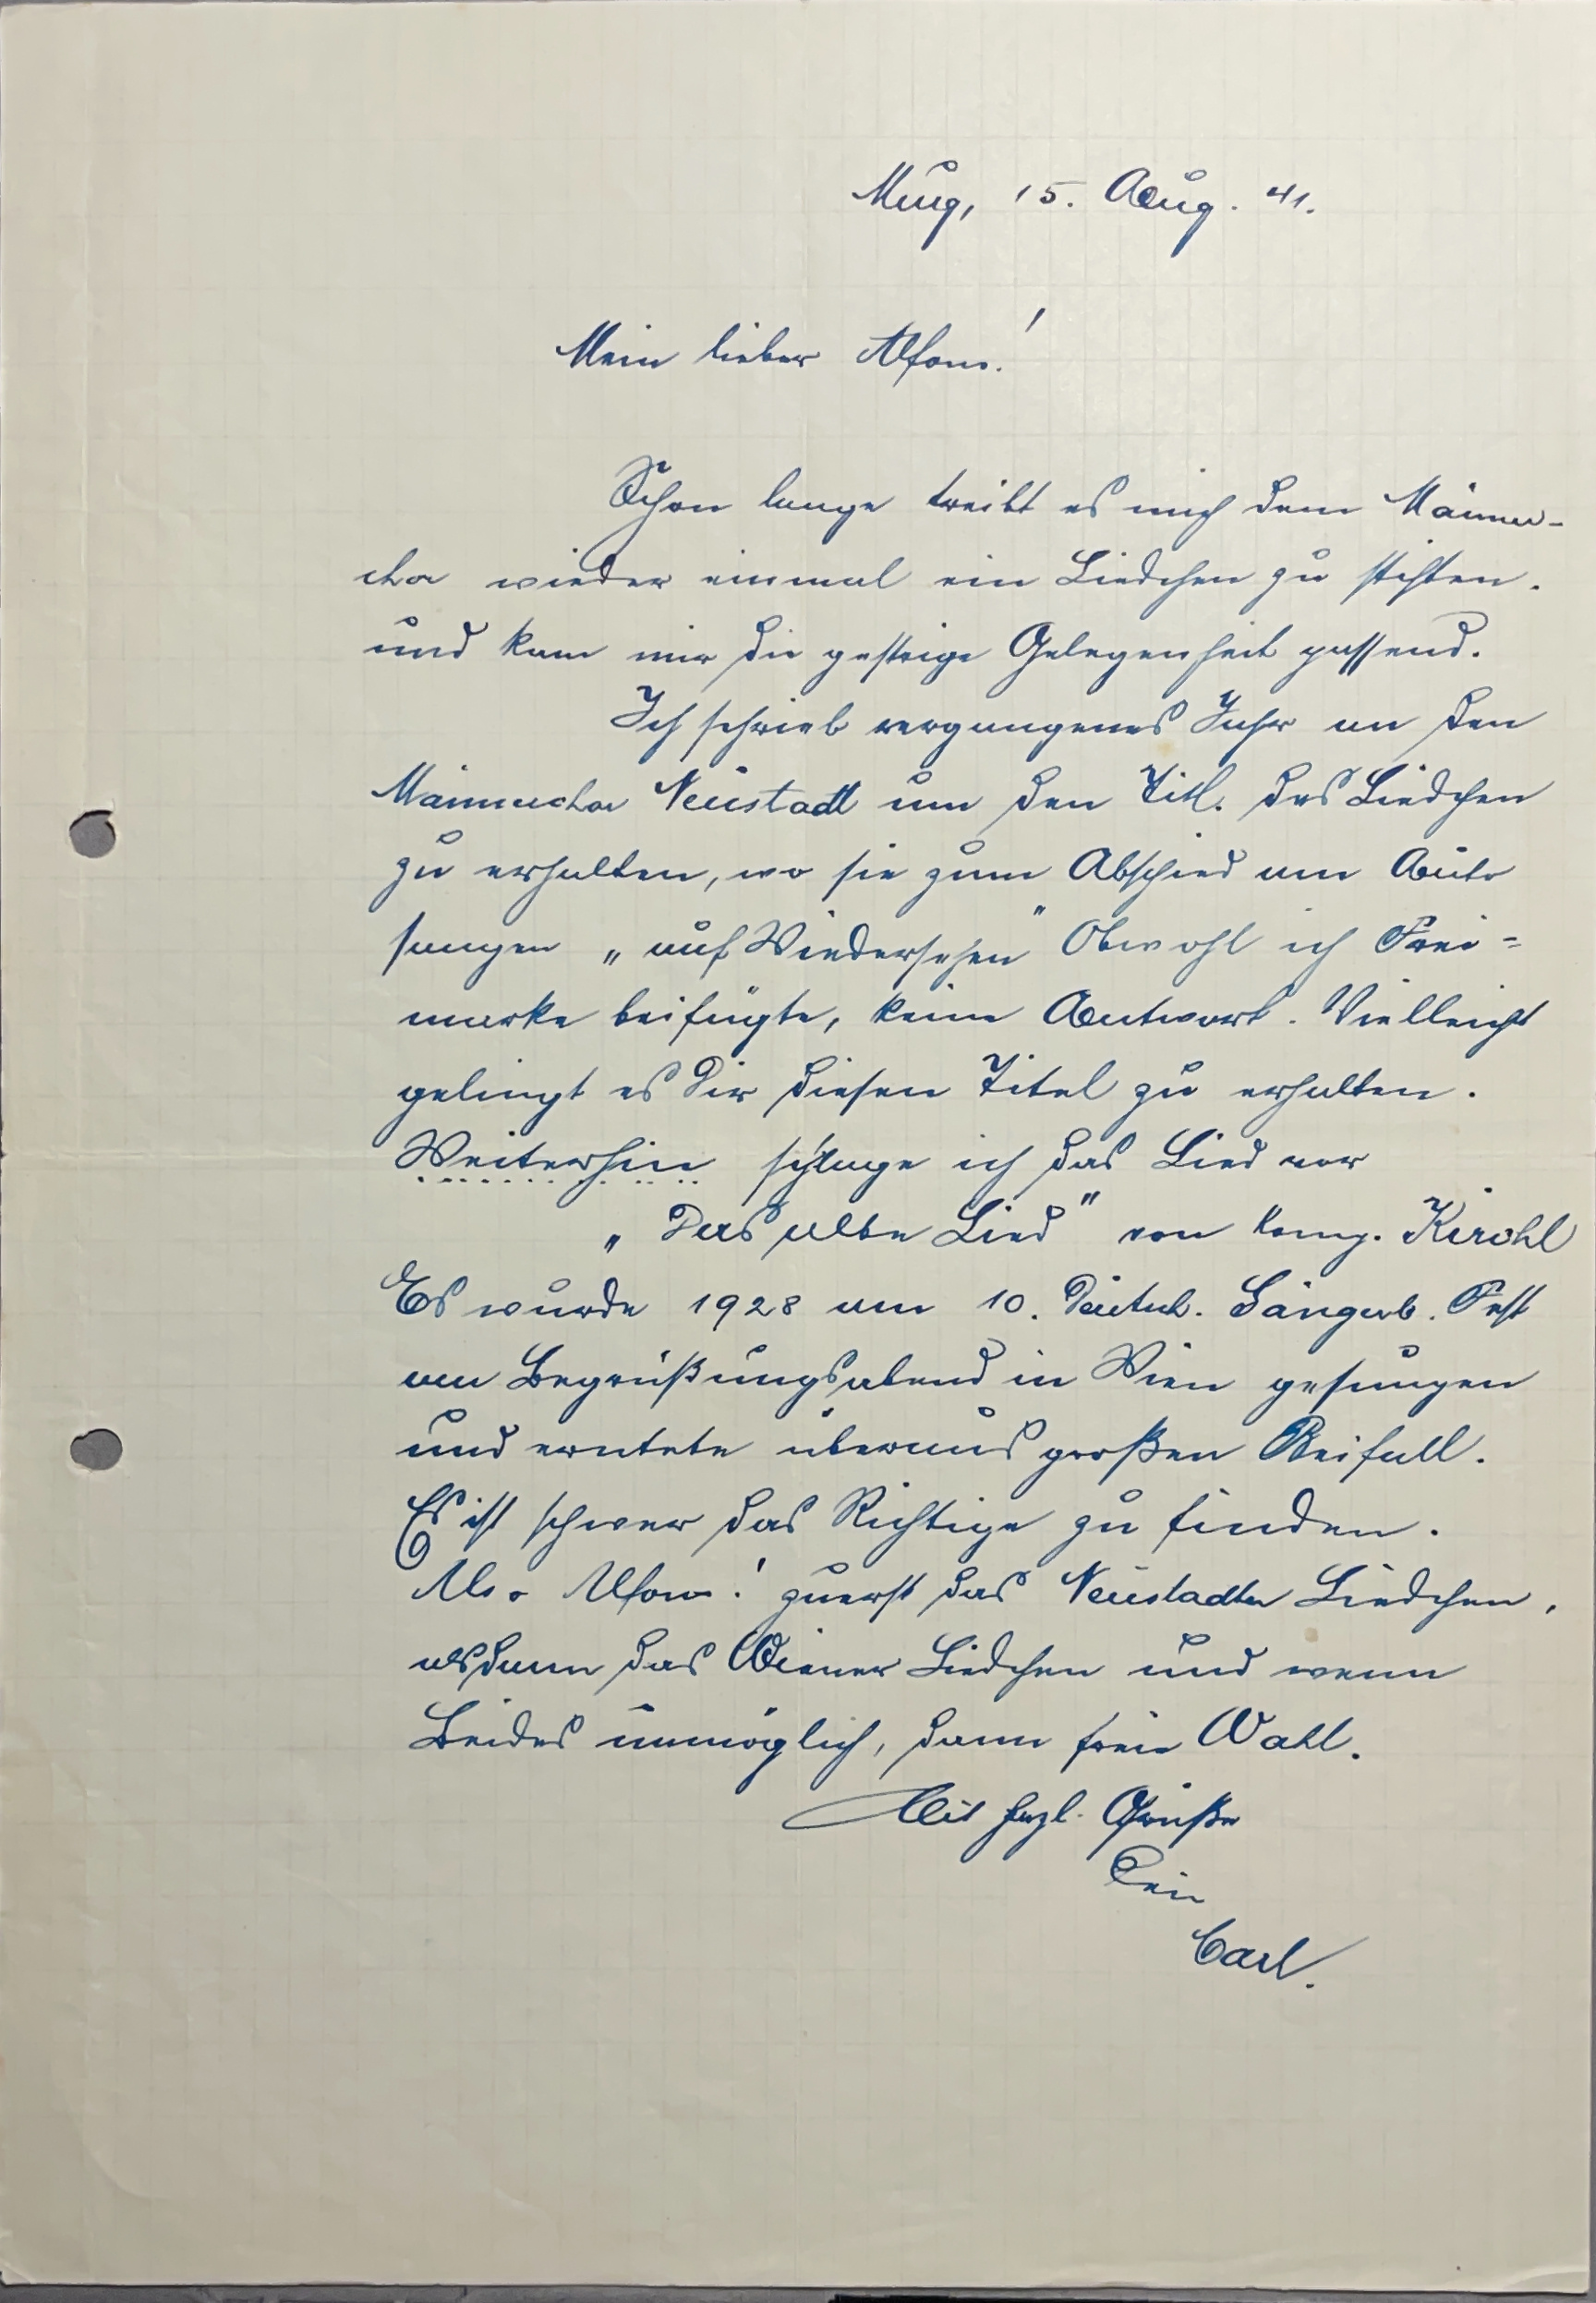
\includegraphics[width=\textwidth]{./assets/Images/Akte_076_S001.jpg}
  \caption{Beispiel für handschriftlichen Text in Akte\_076 erkannt mit Transkribus}
  \label{fig:transkribus-handschrift}
\end{figure}

  \begin{figure}[htbp]
  \centering
  \begin{tcolorbox}[colback=oldLetter, colframe=black, sharp corners, width=\textwidth]
    Murg. 15. Aug 41 

    
    Mein lieber Alfons! 

    Sehen lunge Lreitt es mich dem Männer- 

    chor wieder einmal ein Liedehen zu stehten. 

    und kam mir die gestege Gelegenheit gussend. 

    Männechor Venstad um den Title das Liedchen 

    zu erhalten, wo sie zum Abschied am Aute 

    sängen „auf Wiederschen Owohl ich Frei! 

    märke beifügte, keine Aentwarb. Vielleicht 

    gelingt es Dir diesen Iitel zu erhalten. 
    
    Weiterhin sänge ich fal Lied nur 
    
    ``Bas alte Lied'' von being. Rerohl 

    Es wurde 1928 am 10. Dachub. Sängerb. Frst 

    von Begrüssungsabend in Dien gesungen. 

    und erntete überaus grossen Reifall. 

    Es ich schwer das Richtige zu finden. 

    Aler Alfon, werst das Vemsladler Liedchen. 

    alsdann das Biener Lidchen und wenn 

    Leides unmöglich, dann freu Nall. 

    Mit herzl. Grüsse 

    Dein 

    Carl 
  \end{tcolorbox}
  \caption{Transkription von \autoref{fig:transkribus-handschrift}}
  \label{fig:transkription-brief}

\end{figure}

ChatGPT produziert daraus:

\begin{tcolorbox}[colback=oldLetter, colframe=black, sharp corners, width=\textwidth]
Murg, 15. Aug. 41

Mein lieber Alfons!

Schon lange treibt es mich, dem Männerchor wieder einmal ein Liedchen zu stiften, und kam mir die günstige Gelegenheit gelegen.

Ich schrieb vergangenes Jahr an den Männerchor Venstad, um den Titel des Liedchens zu erhalten, das sie zum Abschied am Auto sangen: \enquote{Auf Wiedersehen, o wohl ich frei!}

Ich fügte eine Frankierung bei, erhielt jedoch keine Antwort. Vielleicht gelingt es Dir, diesen Titel zu erhalten.

Weiterhin sang ich das Lied nur \enquote{Das alte Lied von Wien}. Obwohl es am 10. Dezember 1928 beim Sängerbund-Fest von Begrüssungsabend in Wien gesungen wurde und überaus grossen Beifall erntete, ist es schwer, das Richtige zu finden.

Aber Alfons, zuerst das Venstadler Liedchen, dann das Wiener Liedchen und wenn beides unmöglich, dann Fröhlichsein.

Mit herzlichen Grüssen

Dein

Carl
\end{tcolorbox}

\captionof{figure}{Transkription durch ChatGPT von \autoref{fig:transkription-brief}}
\label{fig:brief-carl-alfons}

Durch ChatGPT verliert der Text zwar seine ursprüngliche Formatierung und Zeilenumbrüche, aber wird nun nahezu fehlerfrei lesbar. Nur das \enquote{Venstadler Liedchen} ist eigendlich eines aus \enquote{Neustadt}. Eine anschliessende menschliche Korrektur ermöglicht also den Abgeleich mit dem nun lesbaren Text, und die Korrektur der Transkription.

Korrigiert und getagt lautet der Brief nun:
  \begin{figure}[htbp]
  \centering
\begin{tcolorbox}[colback=oldLetter, colframe=black, sharp corners, width=\textwidth]
  \textbf{\colorbox{place}{\texttt{Murg}}}.  \textbf{\colorbox{date}{\texttt{15. Aug 41}}} \\
\\
Mein lieber  \textbf{\colorbox{person}{\texttt{Alfons}}}!\\
Seit langem treibt es mich dem  \textbf{\colorbox{organization}{\texttt{Männer-}}}\\
\textbf{\colorbox{organization}{\texttt{chor}}} wieder einmal ein Liedchen zu stiften.\\
und kam mir die günstige Gelegenheit passend.\\
Ich schrieb vergangenes Jahr an den\\
Männechor Vorstand um den Titel das Liedchen\\
zu erhalten, wo sie zum Abschied am Auto \\
sangen \enquote{auf Wiederschen} Obwohl ich  \textbf{\colorbox{unclear}{\texttt{Frank-}}}\\
marke beifügte, keine Antwort. Vielleicht\\
gelingt es Dir diesen Titel zu erhalten.\\
Weiterhin sänge ich das Lied nur\\
\enquote{Das alte Lied} von  \textbf{\colorbox{abbrev}{\texttt{Komp.}}}\textbf{\colorbox{person}{\texttt{ Kirchl}}}\\
Es wurde \textbf{\colorbox{date}{\texttt{1928}}} am \textbf{\colorbox{eventTag}{\texttt{10. Deutsch. Sängerb. Fest}}}\\
am Begrüssungsabend in \textbf{\colorbox{place}{\texttt{Wien}}} gesungen.\\
und erntete überaus grossen Beifall.\\
Es ich schwer das Richtige zu finden.\\
Also \textbf{\colorbox{person}{\texttt{Alfons}}}! zuerst das \textbf{\colorbox{place}{\texttt{Neustadter}}} Liedchen.\\
alsdann das \textbf{\colorbox{place}{\texttt{Wiener}}} Liedchen und wenn\\
Beides unmöglich, dann freie Wahl.\\
Mit herzl. Grüssen \\
Dein\\
\textbf{\colorbox{person}{\texttt{Carl}}}\\
\end{tcolorbox}
\caption{Tagging von \autoref{fig:brief-carl-alfons}}
  \label{fig:Tagging-brief-carl-alfons}
\end{figure}


\begin{tcolorbox}[colback=oldLetter, colframe=black, sharp corners, width=\textwidth]
\textbf{\colorbox{place}{\texttt{München}}}, \textbf{\colorbox{date}{\texttt{28.V.1941}}} \\
\\
Lieber \textbf{\colorbox{person}{\texttt{Otto}}}!\\
Nur wer die Sehnsucht kennt weiss was ich leide\\
Ich wandle traurig her in schwarzer Seide.\\
Die Sehnsucht brennt, du bist so fern.\\
Ach lieber \textbf{\colorbox{person}{\texttt{Otto}}}, wie hab ich dich gern.\\
Ich schnitt es gern in alle Rinden.\\
Ach \textbf{\colorbox{person}{\texttt{Otto}}}, wann u. wo kann ich dich finden?\\
Deine dich nie vergessende\\
\textbf{\colorbox{person}{\texttt{Lina Fingerdick}}}\\
\\
An\\
\textbf{\colorbox{person}{\texttt{Herrn Otto Bollinger}}}\\
z.Hd. \textbf{\colorbox{person}{\texttt{Herrn Alfons Zimmermann}}}\\
\textbf{\colorbox{organization}{\texttt{Vereinsführer des Männerchor}}}\\
\textbf{\colorbox{place}{\texttt{Murg}}}\\
\textbf{\colorbox{place}{\texttt{Laufenburg (Baden)}}}\\
\textbf{\colorbox{place}{\texttt{Rhina}}}
\end{tcolorbox}




\subsection{Diagram english}

\vspace{6\baselineskip}


\begin{center}
\resizebox{0.9\textwidth}{!}{
\begin{tikzpicture}[
  module/.style={rectangle, draw=black, fill=blue!10, thick, minimum width=4.5cm, minimum height=1.2cm, align=center},
  process/.style={rectangle, draw=black, fill=orange!20, thick, minimum width=4.8cm, minimum height=1.2cm, align=center},
  source/.style={rectangle, draw=black, fill=green!30!gray!20, thick, minimum width=4.2cm, minimum height=0.7cm, align=center},
  group/.style={draw=gray, dashed, rounded corners, inner sep=0.5cm},
  arrow/.style={-Latex, thick}, arrowboth/.style={<Latex>-<Latex>, thick},
  node distance=0.8cm and 1.6cm
]


% --- Hauptquellen oben ---
\node[source] (transkribus) at (-14.5, 0) {\textbf{app.transkribus.org} \\ Transcription};
\node[process] (dir) at (0, -3.2) {\textbf{File Directory} \\ with XML-Files};
\node[process] (llmpre) at (6, -3.2) {\textbf{llm\_XML\_preprocessing.py}};
\node[process, below=7.5cm of dir] (main) {\textbf{Transkribus\_II\_Test.py} \\ Main Processing};

% ------------------- MODULE (FLOWCHART) ------------------------
\node[module, below=2cm of main] (init) {Initialization \\ (CSV import, matcher)};
\node[module, below=of init]    (xml)  {XML \& Custom Tags \\ Parse, extract\_metadata};


% Referenzpunkt zentriert unter xml
\coordinate (modcenter) at ($(xml.south) + (0,-1.8)$);
\node[module] (roles)   at ($(modcenter) + (-8cm, -0.5)$) {Roles \\ assign, enrich};
\node[module] (persons) at ($(modcenter) + (-2.7cm, -0.5)$) {Persons \\ match, split, enrich};
\node[module] (orgs)    at ($(modcenter) + (2.7cm, -0.5)$)  {Organizations \\ extract, deduplicate};
\node[module] (places)  at ($(modcenter) + (8cm, -0.5)$)  {Places \\ context + combination};
\node[module] (dates)   at ($(modcenter) + (13cm, -0.5)$) {Dates \\ combine\_dates(), count};
\node[module] (events)  at ($(modcenter) + (-13.5cm, -0.5)$)  {Events \\ extract\_events\_from\_xml()};
\node[module, below=1.2cm of persons] (authors) {Authors \& Recipients \\ infer, deduplicate, score};
\node[module] (json)  at ($(modcenter) + (0cm, -7.5cm)$)  {BaseDocument Build \\ + Role Postprocessing};
\node[coordinate] (joinpoint) at ($(json.north) + (0, 1.5cm)$) {};
\node[coordinate] (joinpointxml) at ($(xml.south) + (0, -0.5cm)$) {};
\node[module, below=of json] (save) {Saving \\ JSON per page + total\_json};

% CSV-Quellen
\node[source] (csv1) at ($(transkribus.south) + (0.5, -4.5)$) {\textbf{export-person.csv}};
\node[source, below=0.6cm of csv1] (csv2) {\textbf{export-place.csv}};
\node[source, below=0.6cm of csv2] (csv3) {\textbf{export-roles.csv}};
\node[source, below=0.6cm of csv3] (csv4) {\textbf{export-organisationen.csv}};

\node[group, fit=(csv1)(csv2)(csv3)(csv4), name=nodegoatbox,
  label={[anchor=north west, xshift=-0.5cm, yshift=0.7cm]north west:\texttt{preprocessing: Nodegoat-export}}] {};

\node[group, fit=(transkribus), name=pretranskribusbox,
  label={[anchor=north west, xshift=-0.5cm, yshift=0.7cm]north west:\texttt{preprocessing: Transkribus}}] {};

 %--- Gruppenrahmen für Modulblock ---
\node[group, fit=
  (persons)(authors)(roles)
  (orgs)(dates)(events)
  (places)(joinpoint), name=flowchartbox] {};

% --- Gruppenrahmen um Hauptverarbeitung + Flowchart ---
\node[group, fit=(main)(flowchartbox)(save),
  label={[anchor=north west, xshift=12.5cm, yshift=+0.7cm]north west:\texttt{ Main Processing of the Pipeline}}] {};


% Verbindungen
\draw[arrow] (transkribus.east) -- ++(1.2,0)-- ++(0,-3.2)-- node[pos=0.6, left, font=\small, xshift=-2cm, yshift=1.3cm]{\textit{Export as XML}} (dir.west);  
\draw[arrow] (dir.east) -- (llmpre.west);
\draw[arrow] (llmpre.north) -- ++(0,1.2) -| node[pos=0.5, above, font=\small, xshift=3cm] {\textit{Custom-Tags}} (dir.north);
\draw[arrow] (dir.south) -- (main.north);
\draw[arrow] (main.south) -- (init.north);
\draw[arrow] (init.south) -- (xml.north);

\draw[arrow] (xml.south) -- (joinpointxml.south);
\draw[arrow] (joinpointxml) -- ($(roles.north |- joinpointxml)$) -- (roles.north);
\draw[arrow] (joinpointxml) -- ($(persons.north |- joinpointxml)$) -- (persons.north);
\draw[arrow] (joinpointxml) -- ($(orgs.north |- joinpointxml)$) -- (orgs.north);
\draw[arrow] (joinpointxml) -- ($(places.north |- joinpointxml)$) -- (places.north);
\draw[arrow] (joinpointxml) -- ($(dates.north |- joinpointxml)$) -- (dates.north);
\draw[arrow] (joinpointxml) -- ($(events.north |- joinpointxml)$) -- (events.north);

\draw[arrow, dashed] (persons.south) -- (authors.north);
\draw[arrow] (persons.west) -- (roles.east);
\draw[arrow] (roles.east) -- (persons.west);   
\draw[arrow] (persons.east) -- (orgs.west);
\draw[arrow] (orgs.west) -- (persons.east); 
\draw[arrow] (persons.east) -- (orgs.west);
\draw[arrow] (orgs.west)-- (persons.east)  ;      
\draw[arrow] (orgs.east) -- (places.west);  
\draw[arrow] (places.west) -- (orgs.east);   
             
% Doppelte Pfeile mit definiertem Stil
\draw[arrow] (events.south) -- ($(events.south |- joinpoint)$);
\draw[arrow] ($(events.south |- joinpoint)$) -- (joinpoint);

\draw[arrow] (roles.south) -- ($(roles.south |- joinpoint)$);
\draw[arrow] ($(roles.south |- joinpoint)$) -- (joinpoint);

\draw[arrow] (authors.south) -- ($(authors.south |- joinpoint)$);
\draw[arrow] ($(authors.south |- joinpoint)$) -- (joinpoint);

\draw[arrow] (orgs.south) -- ($(orgs.south |- joinpoint)$);
\draw[arrow] ($(orgs.south |- joinpoint)$) -- (joinpoint);

\draw[arrow] (places.south) -- ($(places.south |- joinpoint)$);
\draw[arrow] ($(places.south |- joinpoint)$) -- (joinpoint);

\draw[arrow] (dates.south) -- ($(dates.south |- joinpoint)$);
\draw[arrow] ($(dates.south |- joinpoint)$) -- (joinpoint);

\draw[arrow] (joinpoint.south) -- (json.north);
\draw[arrow] (json.south) -- (save.north);
\draw[arrow] 
  (nodegoatbox.south) |- ([xshift=-0.4cm]init.west)
  node[pos=0.6, left, font=\small, xshift=2.6cm, yshift=2.8cm]{\textit{delivers Groundtruth}};
\end{tikzpicture}
}
\end{center}
\vspace{6\baselineskip}


\vspace{6\baselineskip}


\begin{center}
\begin{tikzpicture}

% TikZ styles
\tikzset{
  module/.style={rectangle, draw=black, fill=blue!10, minimum width=0.4cm, minimum height=0.2cm},
  highlight/.style={rectangle, draw=black, fill=blue!40, minimum width=0.4cm, minimum height=0.2cm},
  arrow/.style={-stealth, line width=0.15mm},
  arrowboth/.style={stealth-stealth, line width=0.15mm},
  process/.style={rectangle, draw=black, fill=orange!20, thick, minimum width=6cm, minimum height=1cm, align=center},
  large/.style={rectangle, draw=black, fill=blue!10, thick, minimum width=4.5cm, minimum height=1.2cm, align=center}
}
%==========================
% Mini-Diagramm oben rechts
%==========================

\begin{scope}[shift={(9,0)}]
\node at (0, -3.7) {\textit{Above: Overall schema overview}};
\node[module] (init) at (0,0) {};
\node[module] (xml) at (0, -0.5) {};
\node[module]    (events)  at (-2.0, -1.3) {};
\node[module]    (roles)   at (-1.2, -1.3) {};
\node[highlight] (persons) at (-0.4, -1.3) {};
\node[module]    (orgs)    at ( 0.4, -1.3) {};
\node[module]    (places)  at ( 1.2, -1.3) {};
\node[module]    (dates)   at ( 2.0, -1.3) {};
\node[module] (authors)    at (-0.4, -2  ) {};
\node[module] (json)       at (-0,  -2.8 ) {};
\node[module] (save)       at (-0, -3.3  ) {};
\node[coordinate] (joinpoint) at ($(xml.south) + (0, -1.8cm)$) {};
\node[coordinate] (joinpointxml) at ($(xml.south) + (0, -0.3cm)$) {};

\draw[arrow, dashed] (persons.south) -- (authors.north);
\draw[arrow] (joinpoint.south) -- (json.north);
\draw[arrow] (json.south) -- (save.north);
\draw[arrow] (init.south) -- (xml.north);
\draw[arrowboth] (roles.east) -- (persons.west);
\draw[arrowboth] (persons.east) -- (orgs.west);
\draw[arrowboth] (orgs.east) -- (places.west);
%Pfeile oben
\draw[arrow] (xml.south) -- (joinpointxml.south);
\draw[arrow] (joinpointxml) -- ($(roles.north |- joinpointxml)$) -- (roles.north);
\draw[arrow] (joinpointxml) -- ($(persons.north |- joinpointxml)$) -- (persons.north);
\draw[arrow] (joinpointxml) -- ($(orgs.north |- joinpointxml)$) -- (orgs.north);
\draw[arrow] (joinpointxml) -- ($(places.north |- joinpointxml)$) -- (places.north);
\draw[arrow] (joinpointxml) -- ($(dates.north |- joinpointxml)$) -- (dates.north);
\draw[arrow] (joinpointxml) -- ($(events.north |- joinpointxml)$) -- (events.north);

%Pfeile unten
 Doppelte Pfeile mit definiertem Stil
\draw[arrow] (events.south) -- ($(events.south |- joinpoint)$);
\draw[arrow] ($(events.south |- joinpoint)$) -- (joinpoint);

\draw[arrow] (roles.south) -- ($(roles.south |- joinpoint)$);
\draw[arrow] ($(roles.south |- joinpoint)$) -- (joinpoint);

\draw[arrow] (authors.south) -- ($(authors.south |- joinpoint)$);
\draw[arrow] ($(authors.south |- joinpoint)$) -- (joinpoint);

\draw[arrow] (orgs.south) -- ($(orgs.south |- joinpoint)$);
\draw[arrow] ($(orgs.south |- joinpoint)$) -- (joinpoint);

\draw[arrow] (places.south) -- ($(places.south |- joinpoint)$);
\draw[arrow] ($(places.south |- joinpoint)$) -- (joinpoint);

\draw[arrow] (dates.south) -- ($(dates.south |- joinpoint)$);
\draw[arrow] ($(dates.south |- joinpoint)$) -- (joinpoint);

\draw[arrow] (joinpoint.south) -- (json.north);
\draw[arrow] (json.south) -- (save.north);
\end{scope}

% Large process diagram
\node[large] (personsmod) at (0,0) {\textbf{Persons} \\ match, split, enrich};

\node[process, below=1.2cm of personsmod] (split)  {\textbf{def split\_and\_enrich\_persons} \\ \textit{(Extract raw persons from XML or LLM)}};

\node[process, below=of split] (parse)  {\textbf{def extract\_person\_data} \\ (Split names, detect titles \& role expressions)};

\node[process, below=of parse] (match)  {\textbf{def match\_person} \\ (Fuzzy/contextual matching with groundtruth)};

\node[process, below=of match] (roles)  {\textbf{def assign\_roles\_to\_known\_persons} \\ (Assign roles \& organizations from modules)};

\node[large, right=2.8cm of roles] (rolematch) {\textbf{Role-Matcher.py} \\ (Provides normalized \\ roles)};

\node[large, above=1.3cm of rolematch] (orgmatch) {\textbf{Organization-Matcher.py} \\ (Provides normalized \\ organizations)};

\node[process, below=of roles] (score)  {\textbf{def calculate recipient\_score} \\ (Scoring based on transcript context)};

\node[process, below=of score] (dedup)  {\textbf{def deduplicate\_and\_group\_persons} \\ (Merge persons with same ID/name)};

\node[process, below=of dedup] (count)  {\textbf{def count\_mentions\_in\_transcript\_contextual} \\ (Count mentions in context, avoid duplicates)};

\node[below=of count, align=center] 
  {\textit{Top: process in person\_matcher.py}\\\textit{Right: input from role\_matcher.py and organization\_matcher.py}};

\draw[arrow] (personsmod.south) -- (split.north);
\draw[arrow] (split.south) -- (parse.north);
\draw[arrow] (parse.south) -- (match.north);
\draw[arrow] (match.south) -- (roles.north);
\draw[arrow] (roles.south) -- (score.north);
\draw[arrow] (score.south) -- (dedup.north);
\draw[arrow] (dedup.south) -- (count.north);

\draw[arrow] 
  (orgmatch.west) 
  -- ++(-0.5,0) 
  |- (roles.east);

\draw[arrow] (rolematch.west) -- (roles.east);

\node[draw=gray, dashed, rounded corners, inner sep=0.5cm, fit=(split)(count)] (group) {};
\end{tikzpicture}
\end{center}
\vspace{6\baselineskip}












        \subsubsection{Gründe für den Wechsel zu Nodegoat}
        \subsubsection{Nodegoat Modelierung}


  \subsection{Netzwerkanalyse als Methode}
        \subsubsection{Theoretischer Hintergrund der Netzwerkanalyse}
        \subsubsection{Ziele der Netzwerkanalyse im Kontext der Quellen}
        \subsubsection{Technische Umsetzung (Tools, Datenbankstruktur)}

\newpage
%––––––––––––––––––––––––––––––––––––––––––––––––––––––––––––––––––––––––––––––––––––––%
%––––––––––––––––––––––––––––––––––––––––––––––––––––––––––––––––––––––––––––––––––––––%
%––––––––––––––––––––––––          Aufbau der Datenbank          ––––––––––––––––––––––%
%––––––––––––––––––––––––––––––––––––––––––––––––––––––––––––––––––––––––––––––––––––––%
%––––––––––––––––––––––––––––––––––––––––––––––––––––––––––––––––––––––––––––––––––––––%

     \section{Aufbau der Datenbank}
    \subsection{Konzeption der Datenmodelieung}
      \subsubsection{Eigene Ontologie im Vergleich zu bestehenden Standards}
      \subsubsection{Verknüpfung von Personen, Orten und Ereignissen}
    
    \subsection{Implementierung der Datenbank}
      \subsubsection{Datenbankdesign}
      \subsubsection{Herausforderungen bei der Datenaufnahme}
      \subsubsection{Verknüpfung mit externen Quellen (z.B. Wikidata)}

    \newpage
%––––––––––––––––––––––––––––––––––––––––––––––––––––––––––––––––––––––––––––––––––––––%
%––––––––––––––––––––––––––––––––––––––––––––––––––––––––––––––––––––––––––––––––––––––%
%––––––––––––––––––––––––          Analyse der Netzwerke         ––––––––––––––––––––––%
%––––––––––––––––––––––––––––––––––––––––––––––––––––––––––––––––––––––––––––––––––––––%
%––––––––––––––––––––––––––––––––––––––––––––––––––––––––––––––––––––––––––––––––––––––%
\section{Analyse der Netzwerke}
  \subsection{Soziale Netzwerke des Vereinslebens}
    \subsubsection{Verbindungen zwischen Mitgliedern}
    \subsubsection{ Kooperationen mit anderen Vereinen}
\subsection{ Politische Netzwerke und deren Veränderungen}
    \subsubsection{Einfluss der NS-Diktatur auf die Netzwerke}
    \subsubsection{Feldpostkarten als Quelle für militärische Netzwerke}
    
 \subsection{ Geografische Ausdehnung der Netzwerke}
  \subsubsection{Einsatzorte der Chormitglieder während des Krieges}
  \subsubsection{ Lokale und überregionale Verbindungen}
  \newpage
%––––––––––––––––––––––––––––––––––––––––––––––––––––––––––––––––––––––––––––––––––––––%
%––––––––––––––––––––––––––––––––––––––––––––––––––––––––––––––––––––––––––––––––––––––%
%––––––––––––––––––––––––          Diskussion der Erebnisse      ––––––––––––––––––––––%
%––––––––––––––––––––––––––––––––––––––––––––––––––––––––––––––––––––––––––––––––––––––%
%––––––––––––––––––––––––––––––––––––––––––––––––––––––––––––––––––––––––––––––––––––––%
\section{Diskussion der Ergebnisse}
  \subsection{Sichtbarmachung der Netzwerke durch Nodegoat und Netzwerkanalyse}
  \subsection{Gibt es Veränderungen der Netzwerke im historischen Kontext?}
  \newpage
\endgroup
%––––––––––––––––––––––––––––––––––––––––––––––––––––––––––––––––––––––––––––––––––––––%
%––––––––––––––––––––––––––––––––––––––––––––––––––––––––––––––––––––––––––––––––––––––%
%––––––––––––––––––––––––           Bibliographie         –––––––––––––––––––––––––––––%
%––––––––––––––––––––––––––––––––––––––––––––––––––––––––––––––––––––––––––––––––––––––%
%––––––––––––––––––––––––––––––––––––––––––––––––––––––––––––––––––––––––––––––––––––––%
\pagecolor{white}
\section{Bibliographie}


\begingroup
\small
\singlespacing
\printbibliography[
heading=bibintoc,
title={References}%title of the 'references' section, change this if necessary
]
\endgroup

\newpage
\appendix
\section{Anhang}
\begingroup
\small
\subsection{PDF\_to\_JPEG.py}\label{section:PDF_to_JPEG}
\begin{minted}[
frame=lines,
framesep=2mm,
baselinestretch=1.2,
bgcolor=LightGray,
fontsize=\footnotesize,
linenos,
breaklines=true,  %Automatischer Zeilenumbruch
breakanywhere=true % Minted darf überall umbrechen (optional)
]{python}
import os
import fitz  # PyMuPDF

def convert_pdf_to_jpg(src_folder, dest_folder):
    # Überprüfen, ob der Zielordner existiert, und ihn ggf. erstellen
    if not os.path.exists(dest_folder):
        os.makedirs(dest_folder)

    # Durchgehen durch alle Dateien im Quellordner
    for root, dirs, files in os.walk(src_folder):
        for file in files:
            # Überprüfen, ob die Datei eine PDF-Datei ist
            if file.lower().endswith(".pdf"):
                # Vollständigen Pfad zur PDF-Datei erstellen
                pdf_path = os.path.join(root, file)
                # PDF-Datei öffnen
                doc = fitz.open(pdf_path)
                # Durch alle Seiten der PDF-Datei gehen
                for page_num in range(len(doc)):
                    page = doc[page_num]
                    # Seite in ein PixMap-Objekt umwandeln (für die Konvertierung in JPG)
                    pix = page.get_pixmap()
                    # Dateinamen ohne Dateiendung extrahieren
                    filename_without_extension = os.path.splitext(file)[0]
                    # Ausgabedateinamen erstellen mit führenden Nullen für die 
                    # Seitennummer
                    output_filename = f"{filename_without_extension}_S{page_num + 1:03d}.jpg"


                    # Vollständigen Pfad zur Ausgabedatei erstellen
                    output_path = os.path.join(dest_folder, output_filename)
                    # Bild speichern
                    pix.save(output_path)
                # PDF-Datei schliessen
                doc.close()
                
                # Erfolgsmeldung ausgeben
                print(f"{file} wurde erfolgreich umgewandelt und gespeichert
                in {dest_folder}")

# Pfade zu den Ordnern mit den PDF-Dateien (Quelle) und den JPG-Dateien (Ziel)
src_folder = r"/Users/svenburkhardt/Documents/D_Murger_Männer_Chor_Forschung/Scan_Männerchor/Männerchor_Akten_1925–1945/Scan_Männerchor_PDF"
dest_folder = r"/Users/svenburkhardt/Documents/D_Murger_Männer_Chor_Forschung/Masterarbeit/JPEG_Akten_Scans"


# Funktion aufrufen, um die Konvertierung durchzuführen
convert_pdf_to_jpg(src_folder, dest_folder)

\end{minted}
\subsection{Tagging in Transkribus}


    Transkribus und seine Modelle unterstützen nicht nur beim Transkribieren der Texte, sondern erlauben auch das Taggen von \textit{Named Entities}.  
    Für die vorliegende Arbeit sind dabei besonders Personen, Orte, Organisationen und Daten relevant.  
    Um hierfür ein stringentes Verfahren zu entwickeln, wurden die Tags wie folgt definiert:
    
    \begin{description}

    % Abbreviations
    \item \textbf{\colorbox{abbrev}{\texttt{abbrev}}}
        
    Mit dem Tag \texttt{\texttt{\textbf{{\colorbox{abbrev}{abbrev}}}}} werden alle Abkürzungen getaggt, die für eine eindeutige Entität stehen. 
    
    \noindent\textbf{\ding{43} Beispiel 1}: Dr., Prof., St., Hr., Frl., Dipl.-Ing., etc.
    
    \textbf{\ding{43} Beispiel 2}: Organisationskürzel, wenn sie eindeutig sind: 
    \colorbox{VeryLightGray}{\textless abbrev\textgreater V.D.A.\textless /abbrev\textgreater}.

    \textbf{\textbf{\ding{43} Beispiel 3}}: Falls eine dazugehörige Entität vorhanden ist, wird die Abkürzung getaggt und wird gleichzeitig als zugehörige Entität getaggt:
    
    \colorbox{VeryLightGray}{\textless person\textgreater \textless abbrev\textgreater Dr.\textless /abbrev\textgreater Weiss{\textless /person\textgreater}}

    
    % Unclear    
    \item \textbf{\colorbox{unclear}{\texttt{unclear}}}
    

    Mit dem Tag \texttt{\texttt{\textbf{{\colorbox{unclear}{unclear}}}}} werden unleserliche oder schwer entzifferbare Textstellen markiert. 

    
    \noindent\textbf{\ding{43} Beispiel 1}: Unklare Zeichen oder fehlende Buchstaben: 

    \colorbox{VeryLightGray}{\enquote{Er wohnte in\textless unclear\textgreater [...]\textless unclear\textgreater}.}

    \textbf{\ding{43} Beispiel 2}: Teilweise lesbare Wörter:

    \colorbox{VeryLightGray}{\enquote{{\textless place\textgreater Frei\textless unclear\textgreater [...]\textless unclear\textgreater \textless place\textgreater}}.}
    
%Sic   
    \item\texttt{\textbf{{\colorbox{sic}{sic}}}} 

    Mit dem Tag \texttt{sic} werden Wörter markiert, die im Originaltext in einer falschen oder ungewöhnlichen Schreibweise geschrieben wurden. 
    
    \noindent\ding{43} Beispiel 1: Veraltete oder falsche Schreibweisen: 

    \colorbox{VeryLightGray}{\enquote für dass.}

    \ding{43} Beispiel 2: Offensichtliche Tippfehler, wenn sie im Originaltext so vorkommen: 

    \colorbox{VeryLightGray}{\enquote{Wir haben {<sic>einen</sic>} grosse Freude.}}

    \ding{43} Beispiel 3: Falls eine Korrektur notwendig ist, kann sie als Kommentar ergänzt werden. 

    \end{description}

    \subsubsection{Inhaltliche Tags}
    \begin{description}
    % Person
    \item\texttt{\textbf{{\colorbox{person}{person}}}}
        
    Mit dem Tag \texttt{\colorbox{person}{person}} sollen alle Strings getaggt, die eine direkte Zuordnung einer Person ermöglichen.
    
    \noindent \textbf{\ding{43} Beispiel 1}: Vereinsführer, Alfons, Zimmermann, Alfons Zimmermann, Z. A. Zimmermann, Herr Zimmermann, Herr Alfons Zimmermann, etc. 

    \textbf{\ding{43} Beispiel 2}: Funktionen wie Oberlehrer, Chorleiter, etc.
    Wenn Ort, Name oder Organisation bekannt sind. Eine Person kann sowohl mit ihrem Namen als auch ihrer Funktion (wie Dirigent) getaggt werden.  
    Aus der Korrespondenz ist in der Regel eine zugehörige Organisation ersichtlich, mit deren Verknüpfung eine namentlich nicht genannte Person identifiziert werden könnte.

    
    % Signature    
    \item\texttt{\textbf{{\colorbox{signature}{signature}}}}
        
    Mit dem Tag \texttt{\colorbox{signature}{signature}} werden alle Strings getaggt, die eine handschriftliche Unterschrift darstellen.  
    Der Tag \texttt{\colorbox{signature}{signature}} ist nahezu deckungsgleich mit dem Tag \texttt{\colorbox{person}{person}}.  
    Er dient zur \textbf{graduellen Unterscheidung}, ob ein Name im Fliesstext als gesichert leserlich oder handschriftlich als Signatur vorliegt.  
    
    \noindent \textbf{\ding{43} Beispiel 1}: Eindeutig lesbare Signaturen werden direkt getaggt:  

    \colorbox{VeryLightGray}{\texttt{\textless signature\textgreater A. Zimmermann\textless /signature\textgreater}}. 

    \textbf{\ding{43} Beispiel 2}: Teilweise unleserliche Signaturen werden mit dem Tag \texttt{\colorbox{unclear}{unclear}} innerhalb von \texttt{\colorbox{signature}{signature}} markiert: 

    \colorbox{VeryLightGray}{\texttt{\textless signature\textgreater R. We\textless unclear\textgreater [\ldots]\textless /unclear\textgreater\textless /signature\textgreater}}. 

    
    \textbf{\ding{43} Beispiel 3}: Wenn nur ein Teil des Namens lesbar ist, aber eine Identifikation unsicher bleibt, sollte die Unterschrift vollständig im Tag \texttt{\colorbox{unclear}{unclear}} innerhalb von \texttt{\colorbox{signature}{signature}} stehen:

    \colorbox{VeryLightGray}{\texttt{\textless signature\textgreater \textless unclear\textgreater \textit{etwas unleserliches}\textless /unclear\textgreater \textless /signature\textgreater}.} 
    
    \textbf{\ding{43} Beispiel 4}: Wenn eine Signatur einer bekannten Person zugeordnet werden kann, aber nicht vollständig lesbar ist, bleibt die Signatur erhalten und wird \textbf{ohne} den Tag \texttt{\colorbox{person}{person}} zu verwenden: 

    \colorbox{VeryLightGray}{\texttt{\textless signature\textgreater A. Zimm\textless unclear\textgreater [...]\textless /unclear\textgreater\textless /signature\textgreater}.} 
    
    \textbf{\ding{43} Beispiel 5}: Wenn eine Unterschrift vollständig transkribiert wurde und die Person bekannt ist, wird sie nur mit \texttt{\colorbox{signature}{signature}} getaggt, \textbf{ohne} den Tag \texttt{\colorbox{person}{person}} zu verwenden:  

    \colorbox{VeryLightGray}{\texttt{\textless signature\textgreater Alfons Zimmermann\textless /signature\textgreater}.} 
    
    % Organization    
    \item\texttt{\textbf{{\colorbox{organization}{organization}}}}
        
    Mit dem Tag \texttt{\colorbox{organization}{organization}} werden alle Strings getaggt, die eine direkte Zuordnung einer Organisation ermöglichen.  
    
    \noindent \textbf{\ding{43} Beispiel 1}: Männerchor Murg, Verein Deutscher Arbeiter (V.D.A.), Murgtalschule, etc.

    \textbf{\ding{43} Beispiel 2}: Abkürzungen, wenn sie eine Organisation eindeutig bezeichnen, z.B. V.D.A., NSDAP, STAGMA, etc.
    

    % Place    
    \item\texttt{\textbf{{\colorbox{place}{place}}}}
        
    Mit dem Tag \texttt{\colorbox{place}{place}} werden alle Strings getaggt, die sich auf einen geografischen Ort beziehen.  
    
    \noindent \textbf{\ding{43} Beispiel 1}: Murg (Baden), Freiburg, Berlin, Murgtal, Schwarzwald, etc.

    \textbf{\ding{43} Beispiel 2}: Orte mit näherer Bestimmung, z.B. \enquote{bei Berlin}, \enquote{im Murgtal} werden getaggt:  

    \colorbox{VeryLightGray}{\texttt{\textless place\textgreater im Murgtal\textless /place\textgreater}.} 

    
    % Date    
    \item\texttt{\textbf{{\colorbox{date}{date}}}}
        
    Mit dem Tag \texttt{\colorbox{date}{date}} werden alle expliziten und implizierten Datumsangaben markiert.  
    
    \noindent \textbf{\ding{43} Beispiel 1}:  29.05.1936

    \textbf{\ding{43} Beispiel 2}: 29. Mai 1936

    \textbf{\ding{43} Beispiel 3}: den 29. d. Mts.:

    \colorbox{VeryLightGray}{\texttt{\textless date when=\enquote{29.05.1936}\textgreater den 2.\textless /date\textgreater} \texttt{\textless abbrev\textgreater d. Mts.\textless /abbrev\textgreater}}

% Event
    \item\texttt{\textbf{{\colorbox{eventTag}{event}}}}
    
    Mit dem Tag \texttt{\colorbox{eventTag}{event}} werden expliziten und implizierten Ereignisse markiert. Diese Ereignisse haben einen zeitlichen oder räumlichen Bezug, und können benannt werden. Dazu zählen:

    \noindent \textbf{\ding{43} Beispiel 1}: \enquote{Jubiläumskonzert}

    \textbf{\ding{43} Beispiel 2} \enquote{Gründung des Vereins} 

    \textbf{\ding{43} Beispiel 2}\enquote{Kriegsausbruch} oder \enquote{Kriegsende}

    Konzepte, die nicht klar in den Texten benannt werden, wie beispielsweise die Suche nach einem Dirigenten, können nicht immer Ereignis getaggt werden. Sie sollen später aber in der Datenbank implementiert werden.
    \end{description}
    
    \subsubsection{Strukturelle Tags}
    \begin{description}

    % Abbreviations
    \item\texttt{\textbf{{\colorbox{abbrev}{abbrev}}}}
    
        
    Mit dem Tag \texttt{\texttt{\textbf{{\colorbox{abbrev}{abbrev}}}}} werden alle Abkürzungen getaggt, die für eine eindeutige Entität stehen.

    
    \noindent\textbf{\ding{43} Beispiel 1}: Dr., Prof., St., Hr., Frl., Dipl.-Ing., etc.

    \textbf{\ding{43} Beispiel 2}: Organisationskürzel, wenn sie eindeutig sind:\\\colorbox{VeryLightGray}{\textless abbrev\textgreater V.D.A.\textless /abbrev\textgreater}.

    \textbf{\textbf{\ding{43} Beispiel 3}}: Falls eine dazugehörige Entität vorhanden ist, wird die Abkürzung getaggt und wird gleichzeitig als zugehörige Entität getaggt:

    \colorbox{VeryLightGray}{\textless person\textgreater \textless abbrev\textgreater Dr.\textless /abbrev\textgreater Weiss{\textless /person\textgreater}}
    
    % Unclear    
    \item\texttt{\textbf{{\colorbox{unclear}{unclear}}}}
    

    Mit dem Tag \texttt{\texttt{\textbf{{\colorbox{unclear}{unclear}}}}} werden unleserliche oder schwer entzifferbare Textstellen markiert.
    
    \noindent\textbf{\ding{43} Beispiel 1}: Unklare Zeichen oder fehlende Buchstaben: 

    \colorbox{VeryLightGray}{\enquote{Er wohnte in\textless unclear\textgreater [\ldots]\textless unclear\textgreater}.}

    \textbf{\ding{43} Beispiel 2}: Teilweise lesbare Wörter:

    \colorbox{VeryLightGray}{\enquote{{\textless place\textgreater Frei\textless unclear\textgreater [\ldots]\textless unclear\textgreater \textless place\textgreater}}.}

    
%Sic   
    \item\texttt{\textbf{{\colorbox{sic}{sic}}}} 

    Mit dem Tag \texttt{sic} werden Wörter markiert, die im Originaltext in einer falschen oder ungewöhnlichen Schreibweise geschrieben wurden.

    \noindent\ding{43} Beispiel 1: Veraltete oder falsche Schreibweisen: 

    \colorbox{VeryLightGray}{\enquote für dass.}

    \ding{43} Beispiel 2: Offensichtliche Tippfehler, wenn sie im Originaltext so vorkommen: 

    \colorbox{VeryLightGray}{\enquote{Wir haben {<sic>einen</sic>} grosse Freude.}}

    \ding{43} Beispiel 3: Falls eine Korrektur notwendig ist, kann sie als Kommentar ergänzt werden. 

    \end{description}



    \endgroup
\end{document}
